% utf-8 ru, unix eolns
\documentclass[12pt,a4paper,oneside]{extarticle}
    \righthyphenmin=2 %минимально переносится 2 символа %%%
    \sloppy

\usepackage{style}

\begin{document}

    \section{Вопросы}
        \begin{itemize}

            \item Не лучше ли "поверхностную" постановку задачи расположить во введении, а подробное описание сделать в начале главы реализация?
            \item Перевод bridging vocabulary (в контексте это примерно значит: связующие словари или перекрывающие)
            \item вставить в реализацию описание оборудования и софта
        \end{itemize}
    \clearpage


    \pgfplotsset{compat=1.8}

\thispagestyle{empty}
\newpage
{
\centering


\textbf{
МОСКОВСКИЙ ГОСУДАРСТВЕННЫЙ ТЕХНИЧЕСКИЙ УНИВЕРСИТЕТ ИМЕНИ Н. Э. БАУМАНА \\
Факультет информатики и систем управления \\
Кафедра теоретической информатики и компьютерных технологий}
\bigskip
\bigskip
\bigskip
\bigskip
\bigskip
\bigskip
\bigskip

\vfill

Курсовой проект \\
по курсу <<Конструирование компиляторов>>

\bigskip

{\large <<Препроцессор синаксического сахара для языка Scheme>>}
\bigskip

\vfill



\hfill\parbox{4cm} {
Выполнил:\\
студент ИУ9-101 \hfill \\
Выборнов А. И.\hfill \medskip\\
Руководитель:\\
Дубанов А. В.\hfill
}


\vspace{\fill}

Москва \number\year
\clearpage
}

    %\section*{Аннотация}
\summarytitle

В данной работе рассматривается применение методов машинного обучения и обработки естественного языка к решению задачи автоматической связи сообщений твиттера и новостных статей.

Проведен обзор существующих подходов к решению задачи.
Проведено исследование эффективности различных методов решения задачи и разных способов построения набора данных.
Реализовано автоматическое установления связей между сообщениями твиттера и новостными статьями в формате рекомендаций для твита наиболее подходящих новостных статей.

В организационно-экономической части представлено технико-экономическое обоснование разработки, проанализирована структура затрат проекта и построен календарный план-график проекта.

Пояснительная записка к работе содержит текст на \pageref{LastPage} листах формата А4,  \totfig~таблиц, \tottab~рисунков, список литературы из \totbibref~библиографических ссылок.
%К данной работе разработана презентация в формате *.pdf из ... слайдов.
\thispagestyle{empty} \clearpage
    \tableofcontents \clearpage
    \section*{Введение}
\addcontentsline{toc}{section}{Введение}
    В современном мире всё больший вес приобретают социальные медиа~(преимущественно социальные сети).
    Их главное отличие от традиционных медиа (газеты, тв) заключается в том, что контент порождается тысячами и миллионами людей.
    Социальные медиа не заменяют традиционные новостные источники, а дополняют их.
    Они могут служить полезным социальным датчиком того, насколько популярна история~(тема) и насколько долго.
    Часто, обсуждения в социальных медиа основаны на событиях из новостей и, наоборот, социальные медиа влияют на новостные события.

    Одной из самых популярных социальных сетей является Twitter~(Твиттер)~---~социальная сеть для публичного обмена сообщениями.
    Главной особенностью Твиттера является малый размер сообщений~(140 символов), называемых твитами.
    Часто твиты являют собой описание происходящего прямо сейчас события, отклик на него.

    Происходящие в мире события описываются статьями в новостных изданиях.
    Новостные статьи и твиты пользователей твиттера не редко описывают одно и то же событие.
    Существует актуальная проблема установления связей между твитами и новостными статьями, которые описывают одно и тоже событие.
    Выявление связи между сообщениями твиттера и новостями позволит как расширить информативность твитов, так и обогатить новости.

    Среди преимуществ расширения новости с помощью твитов можно выделить такие, как определение отношения аудитории к новости,
    дополнительные признаки для тематической классификации новостей, дополнительная информация для аннотирования новостей.

    Современные методы обработки естественного языка хорошо работают, используя большой массив текста в качестве входных данных, однако, они становятся неэффективными,
    когда применяются на коротких текстах, таких как твиты.
    Существенным преимуществом расширения твита с помощью новости является появляющаяся возможность использования большого количества методов обработки естественного языка.

    Данная работа ставит целью исследование и разработку методов автоматического установления связей между сообщениями твиттера и новостными статьями.

    \clearpage \clearpage
    \section{Обзор}
    В двух словах о решаемой задаче.

    О том, что задача похожа на поиск семантического сходства между короткими текстами. Она плохо решаема.

    \subsection{Терминология}
    Решение задачи предполагает использование наработок различных дисциплин, таких как: обработка естественного языка, машинное обучение, информационный поиск,
    а основным источником данных выступают интернет ресурсы.
    Поэтому в работе используется специфичная терминология.

    \textit{Твиттер}~---~cоциальная сеть для публичного обмена короткими~(до 140 символов) сообщениями при помощи веб-интерфейса, SMS,
    средств мгновенного обмена сообщениями или сторонних программ-клиентов.

    \textit{Твит}~---~термин сервиса микроблоггинга Твиттер, обозначающий сообщение, публикуемое пользователем в его твиттере.
    Особенностью твита является его длина, которая не может быть больше 140 знаков.

    \textit{Ретвит}~---~сообщение, целиком состоящее из цитирования сообщения одного пользователя Твиттера другим.

    \textit{Новость}~---~оперативное информационное сообщение, которое представляет политический, социальный или экономический интерес для аудитории в своей свежести,
    то есть сообщение о событиях произошедших недавно или происходящих в данный момент.

    \textit{Хэштег}~---~слово или фраза, которым предшествует символ \#, используется в различных социальных сетях~(Twitter, Facebook, Instagram)
    для объединения группы сообщений по теме или типу.
    Например: \#искусство, \#техника, \#смешное, \#анекдоты и т.д.

    \textit{URL}~(от англ. Uniform Resource Locator~---~единый указатель ресурса)~---~единообразный определитель местонахождения ресурса.
    URL служит стандартизированным способом записи адреса ресурса в сети Интернет.

    \textit{Обработка естественного языка}~(англ. Natural language processing)~---~направление математической лингвистики,
    которое изучает проблемы компьютерного анализа и синтеза естественных языков.

    \textit{Именованная сущность}~---~последовательность слов, являющаяся именем, названием, идентификатором, временным, денежным или процентным выражением.

    \textit{Аннотирование текста}~---~краткое представление содержания текста в виде аннотации~(обзорного реферата).

    \textit{Информационный поиск}~---~процесс поиска неструктурированной документальной информации, удовлетворяющей информационные потребности, и наука об этом поиске.

    \textit{TF-IDF}~(от англ. TF~---~term frequency, IDF~---~inverse document frequency)~---~статистическая мера, используемая для оценки важности слова в контексте документа,
    являющегося частью коллекции документов или корпуса.
    Вес некоторого слова пропорционален количеству употребления этого слова в документе, и обратно пропорционален частоте употребления слова в других документах коллекции.

    \textit{TF-IDF матрица}~---~матрица, строки которой соответствуют словам из корпуса, а столбцы текстам.
    Значение ячейки матрицы $(i,j)$ равно значению метрики tf-idf для слова, соответствующего строчке $i$, и текста, соответствующего столбцу $j$.

    \textit{WTMF}~---~метод машинного обучения, применяемый для анализа схожести между короткими текстами~\cite{wtmf}.

    \textit{Тематическое моделирование}~---~способ построения модели коллекции текстовых документов, которая определяет, к каким темам относится каждый из документов.

    \textit{LDA}~(от англ. Latent Dirichlet allocation~---~Латентное размещение Дирихле)~---~методов тематического моделирования,
    позволяющий объяснять результаты наблюдений с помощью неявных групп.



%    \textit{Классификация}~---~Это осмысленный порядок вещей, явлений, разделение их на разновидности согласно каким-либо важным признакам.
%
%    \textit{Тематическая модель}~---~модель, которая по коллекции текстовых документов, определяет, к каким темам относится каждый документ и какие слова~(термины) образуют каждую тему.
%
%    \textit{Тональность текста}~---~эмоциональная оценка автора по отношению к объектам, речь о которых идет в тексте.
%

%
%    \textit{Точность}~---~доля релевантных документов выборки по отношению ко всем документам в выборке.
%
%    \textit{Полнота}~---~доля релевантных документов в выборке по отношению ко всем релевантным документам коллекции.



    \subsection{Существующие подходы к решению задачи}
    %мб и не нужна следующая фраза:
    %В рамках предварительного исследования были разобраны несколько статей . Ниже приводится краткое изложение основных идей, описанных в выбранных статьях.
    Задача автоматического установления связей между твитами и новостными статьями пока не имеет устоявшегося решения.
    В рамках предварительного исследования были отобраны наиболее перспективные подходы к решению задачи, а именно:
    \begin{itemize}
        \item Метод WTMT-G, представляющий собой доработку метода WTMF, которая позволила учитывать информацию о связях между текстами. Предложен в статье \cite{linking_base}.
        \item Обобщённый метод, позволяющий по новости находить относящиеся к ней высказывания из социальных медиа. Предложен в статье \cite{linking_news_media}
        \item Связывание твитов с новостями на основе bridging словарей \textcolor{red}{(нужен перевод слова bridging, в конктексте это примерно значит: связующие словарии или перекрывающие)}. Предложен в статье \cite{bridging}.
    \end{itemize}
    Также рассматривается классическое решение задачи поиска похожих текстов на основе частотности употребления слов.
    Ниже представлен краткий обзор выбранных методов.

    \subsubsection{Поиск похожих текстов на основе частотности употребления слов}
        описание рекомендаций на основе tfidf

    \subsubsection{WTMF-G}
        по статье Linking Tweets to News: A Framework to Enrich Short Text Data in Social Media

        В двух-трёх абзацах описание подхода, описание задачи убрать.

        \paragraph{Перевод аннотации}
            Многие современные методы обработки естественного языка~(NLP\footnote{Natural Language Processing}) хорошо работают с большой массив текста в качестве входных данных.
            Однако они очень неэффективными при работе с короткими текстами (к примеру твиты).
            Преодоление этой проблемы мы видим в нахождении соответствующего твиту новостного документа.
            Решение этой задачи требует хорошего моделирования семантики коротких текстов.

            Основной вклад статьи двойной:
            \begin{enumerate}
                \item представлено решение задачи нахождения взаимосвязи между твитами и новостями, из этого могут извлечь выгоду многие NLP задачи;
                \item в отличие от предыдущих исследований, которые фокусируются на лексических особенностях коротких текстов~(информация о связи текст-слово), мы предлагаем взаимосвязь, основанную на модели скрытой переменной, которая моделирует корреляцию между короткими текстами~(информация о связи текст-текст). Необходимость этого обоснована наблюдением: твит обычно покрывает только один аспект события.
            \end{enumerate}

            Мы покажем, что c помощью особенных признаков твита~(хэштегов) и особых признаков новостей~(именнованных сущностей\footnote{Какой-то кривой перевод, найдо найти получше. In data mining, a named entity is a phrase that clearly identifies one item from a set of other items that have similar attributes.}) а также временн\'{ы}х ограничений, мы можем получить взаимосвязь текст-текст, и, таким образом, дополнить семантическую картину короткого текста.
            Наши эксперименты показывают значительное преимущество нашей новой модели над baseline\footnote{Как перевести?}.

        \paragraph{Идея статьи}
            Современные методы обработки естественного языка плохо работают с короткими текстами. Для преоболения этого к твитам привязываются соответствующие новости.

            Для формирования обучающей выборки, были выбраны твиты, которые имели ссылки на новости, опубликованные новостными агенствами (CNN или NYT) в тот же период.

            Как показано в статье~\cite{long_to_short}, добавление к твиту содержимого веб-страницы, ссылка на которую включена в этот твит, повышает {\color{red} purity score} их кластеризации с 0.280 до 0.392.

            Модели со скрытой переменной хорошо подходят для отображения коротких текстов в плотный малоразмерный вектор.
            В рамках решения задачи была применена модель со скрытой переменной, которая называется WTMF~(Weighted Textual Matrix Factorization, подробное описание\cite{wtmf}), к твитам и к новостям. Модель была протестирована на двух схожих наборах данных из небольших сообщений. Как результат - используемая модель с большим запасом превзошла и LSA~(Latent Semantic Analysis) и LDA~(Latent Dirichelet Allocation). Эта модель позволила добавить информацию об отсутствующих словах в твит (модель WTMF добавляет более 1000 фичей к твиту, LDA лишь 14). Недостатком WTMF является то, что порождается только связь текст-слово, без учёта взаимосвязи между короткими текстами.

            Ввиду разреженности исходных данных, возникает ещё одна проблема: твит обычно отражает, только один аспект события.

            Полученный подход не учитывает следующих характеристик, которым обладает исходная выборка:
            \begin{enumerate}
                \item Хэштеги, которые являются прямым указанием на смысл твита.
                \item {\color{red} Named entities} новостей. Из новостей можно с высокой точностью извлекать {\color{red} named entities}, используя инструменты для NER~(Named Entity Recognition). Если несколько текстов содержат схожие {\color{red} named entities} они наверняка описывают одно и тоже событие.
                \item Информация о времени публикации для твитов и новостей. Если несколько текстов опубликованы примерно в одно и то же время, то велик шанс, что они описывают одно и тоже событие
            \end{enumerate}
            В статье описывается решение проблемы поиска взаимосвязи между текстами, с использованием описанных выше характеристик. Два связанных текста, должны иметь схожий скрытый вектор (семантическая модель твита достраивается из схожих твитов).

            Это дополнительная информация была добавлена в модель WTMF. Было также показано различное влияние на связь текст-текст жанра твита и жанра новости. Был получен на порядок более лучший результат чем при использовании исходной WTMF модель.

    \subsubsection{Обобщённый метод, сопоставляющий новости высказывания из социальных медиа}
        по статье Linking Online News and Social Media

        В двух-трёх абзацах описание подхода, описание задачи убрать.

        \paragraph{Перевод аннотации}
            Многое из того, что обсуждается в социальных медиа вдохновлено событиями, описанными в новостях и, наоборот, социальные медиа предоставляют механизм, позволяющий влиять на новостные события.
            Мы обращаемся к следующей задаче: по новости, найти в социальных сетях высказывания, которые неявно на неё ссылаются.
            Используется трехступенчатый подход: сначала получаются несколько моделей запросов по исходной статье, затем модели используются для получения высказываний из индекса целевого социального медиа, результатом являются несколько ранжированных списков, которые объединяются с использованием особой техники слияния данных.
            Модель запроса создаётся как на основе структуры статьи, так и на основе явно связанных со статьей высказываний из социальных медиа.
            Для борьбы с дрейфом запроса\footnote{Порождение менее подходящего запроса.} при большого объёме используемого текста (либо в новости, либо в явно связанных высказываниях из социальных медиа), предлагается основанный на графике метод для выбора отличительных условий.

            В нашей экспериментальной оценки для порождения моделей запросов, использованы данные из Twitter, Digg, Delicious\footnote{Веб-сайт, бесплатно дающий зарегистрированным пользователям услугу хранения и публикации закладок на страницы Всемирной сети.}, the New York Times Community, Wikipedia и блогосферы.
            Показано, что другие модели запросов, основанные на различных источниках данных, не только обеспечивают дополнительную информацию, но и влияют на получение различных высказываний из социальные медиа по нашему целевому индексу.
            Как следствие, методы слияния данных приводят к значительному повышению производительности в сравнении с индивидуальными подходами.
            Показано, что основанный на графике метод выделения условий помог улучшить как эффективность, так и продуктивность.

    \subsubsection{Связывание твитов с новостями на основе bridging словарей}
        Статья Bridging Vocabularies to Link Tweets and News

        В двух-трёх абзацах описание подхода, описание задачи убрать.

        \paragraph{Основная идея}
            Значительную сложность при решении проблемы связывания твитов с новостями преимущественно вызывают малый размер твита и различия в словарях: в твитах используются аббревиатуры, неформальный язык, сленг, в новостях, напротив, используется литературный язык. Также твиты очень зашумлены и не содержать полезного содержимого.

            Твиттер предлагает хештэги, как механизм для категоризации твитов. Но этот подход далеко не совершенен, так как не только далеко не все записи содержат хештеги, но и записи содержащие хeштеги обладают рядом проблем. Такими как: хeштег не содержит информацию о событии, хeштег сформулирован в слишком общей форме, твит содержит несколько хештегов. Из этого делается вывод, что использование только хештегов приведёт к низкому качеству связывания твитов с новостями.

            Предлагается следующий подход:
            Используется LDA для построения моделей тем поверх новостей. Затем среди твитов ищутся наиболее близкие к конкретному топику. Из полученных твитов извлекаются слова, которые служат ``мостом'' к другим твитам.


    \subsection{Метод WTMF-G}
    Построение модели для метода WTMF-G основывается на построение модели метода WTMF.
    Набор данных состоит из множества новостей и твитов и связей вида текст-текст, из которых, в процессе работы извлекается набор текстов.
    ~(для твита~---~текст твита, для новости~---~конкатенация заголовка и краткого изложения статьи).

    По множеству текстов, которые получены из набора данных, построена пригодная для сериализации модель, представляющая собой матрицу $P$.
    Построение модели зависит от четырёх констант:
    \begin{enumerate}
        \item $K$~---~размерность вектора, по которому производится сравнение~
        (если TF-IDF матрица $X$ была размера $M \times N$, то по завершении работы алгоритма будут получены две матрицы $P$ размера $K \times M$ и $Q$ размера $K \times N$);
        \item $I$~---~число итераций алгоритма построения модели;
        \item $w_M$~---~коэффициент, задающий вес негативного сигнала при построении матрицы весов $W$;
        \item $\delta$~---~коэффициент, задающий степень влияния связей вида текст-текст.
    \end{enumerate}

    Применение полученной модели на множество твитов производится аналогично применению модели для метода WTMF за исключением двух моментов:
    во-первых, необходимо на основе новостей из набора данных и множества твитов перестроить связи текст-текст, во-вторых получение матрицы $Q$ происходит по следующей формуле:
    $$Q_{\cdot, j} = (P W'_j P^T + \lambda I + \delta  L_j^2 Q_{\cdot,n(j)} diag(L^2_{n(j)})Q_{\cdot,n(j)}^T)^{-1}   (P W'_j X_{j,\cdot} + \delta  L_j Q_{\cdot,n(j)} L_{n(j)}).$$
    В результате получаем вектора для сравнения твитов из заданного множества.
    \subsection{Оценка качества}
    формулирование того как переходим к рекомендациям и что вообще в них меряем

    \subsubsection{RR}
        описание метрики
    \subsubsection{TOP10}
        описание метрики
    \subsubsection{ATOP}
        описание метрики и обоснование почему она не очень

        Используем метрику $ATOP$ (метрика подробно описана в \cite{steck_recommender}).
        Рассмотрим что означает эта метрика в применении к нашей задаче (я немного модифицировал метрику, для более простого описания, полученная метрика полностью совпадает с описанной метрикой).
        Пусть $T$ - это множество твитов, $N \in \mathbb{N}$ - размер рассматриваемого топа новостей для твита (могут быть все новости вообще), $k < N \in \mathbb{N}$.
        $TOPK_t(k) = 1$, если твит $t \in T$ соответствует хотя бы одной новости в top-k результатов, иначе $TOPK_t(k) = 0$
        $$TOPK(k) = \dfrac {\sum_{t \in T} TOPK_t(k)} {|T|},$$
        $$ATOP = \dfrac{\sum_{k=1}^N TOPK_t(k)}{N} = \dfrac{1}{|T| * N} \sum_{k=\overline{1,N}, ~t \in T} TOPK_t(k).$$

        Значения метрики $ATOP$ лежат на отрезке $[0,1]$. Чем ближе $ATOP$ к $1$ тем лучше.
    \subsection{Nature Language Processing}
    Всё что связано с обработкой текста

    \subsubsection{Лемматизация}
    \label{subsubsec:lemma}
        что это

        как используется

        https://pythonprogramming.net/stop-words-nltk-tutorial/?completed=/tokenizing-words-sentences-nltk-tutorial/
    \subsubsection{Извлечение имён собственных}
        что это

        Обзор подходов

        объяснение используемого





 \clearpage
    \section{Установления взаимосвязей между новостями и твитами}
    Задача автоматического установления связей между твитами и новостями решена посредством написания программного комплекса,
    который обладает следующими возможностями:
    \begin{enumerate}
        \item сбор необходимой для решения задачи информации;
        \item построение наборов данных;
        \item применение к наборам данных методов машинного обучения;
        \item получение рекомендаций новостей для произвольных твитов;
        \item вариативность в выборе метода для построения рекомендаций;
        \item возможность получить информацию о качестве используемого метода.
    \end{enumerate}
    Программный комплекс реализован с использование языка программирования Python версии 2.7.

    \textcolor{red}{Ниже приводится описание архитектуры программного комплекса, а также разбор отдельных моментов.}

    \subsection{Архитектура}
    Программный комплекс позволяет производить все требуемые для решения задачи преобразования над данными, а именно:
    \begin{enumerate}
        \item получение данных из твиттера;
        \item получение данных из новостной rss-ленты;
        \item расшифровка сокращённых URL;
        \item автоматическое построение набора данных;
        \item построение моделей для методов WTMF и WTMF-G;
        \item построение рекомендаций на основе методов WTMF, WTMF-G и TF-IDF;
        \item оценка качества рекомендаций;
        \item получение результатов рекомендаций в пригодном для чтения формате;
    \end{enumerate}
%    Результаты всех преобразований, за исключением оценки качества и получения рекомендаций, хранятся в специальном промежуточном
%    хранилище~(побробное описания хранилища производится в разделе~\ref{sec:documentation}).

    Каждое преобразование, в общем случае, независимо от других.
    Для построения рекомендаций, необходимо выполнить цепочку преобразований.
    Примеры цепочек преобразований для получения данных, построения рекомендаций и оценки их качества приводятся ниже.
    
    Визуализация цепочек преобразований производится при помощи рисунков, использующих элементы блок-схем~\cite{flowchart_gost}.
    Для удобства восприятия блоки действия~(изображаются прямоугольником) выделяются зелёным цветом, 
    а прочие используемые блоки, такие как ввод-вывод данных~(изображаются параллелограммом) и хранимые 
    данные~(изображаются фигурой, представляющей собой прямоугольник, в котором две противолежащие стороны 
    заменены на две одинаковые и параллельные кривые, совпадающие с секцией окружности), выделяются синим цветом.
    
    Получение данных заключается в скачивании новостей из RSS потоков и твитов, с использованием Twitter Streaming API, в течение длительного промежутка времени, с последующим помещением всех данных в промежуточное хранилище. В работе в качестве хранилища выступает python shelve.
    Получение данных в виде блок-схемы изображен на рисунке~\ref{pic:consumer_flowchart}.
    \begin{figure}[h!]
            \center
            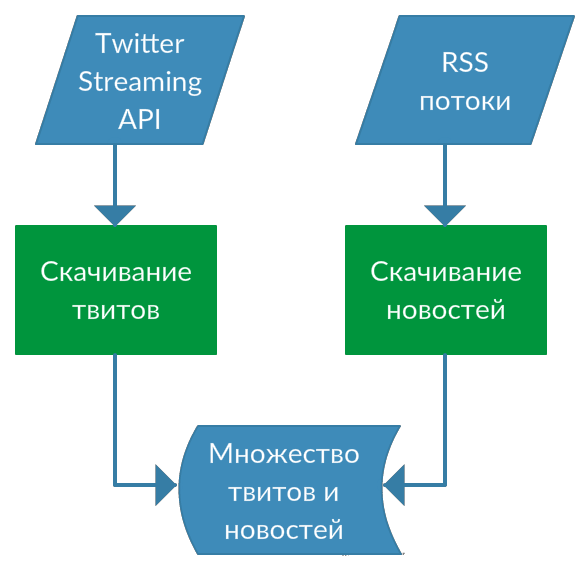
\includegraphics[scale=0.4]{twnews_consumer_flowchart.png}
            \caption{Блок-схема получения данных}
            \label{pic:consumer_flowchart}
    \end{figure}

    На основе полученного множества новостей и твитов происходит автоматическое построение набора данных. В рамках автоматического построения набора данных происходит расшифрка сокращённых URL.
    Набор данных эта структура состоящая из списка новостей и списка твитов, где для каждого твита указана ссылка на единственную новость.

    Результатом работы всех реализованных методов является сопоставление численных векторов~(векторов для сравнения) каждому обрабатываемому тексту, с помощью которых можно оценить насколько похожи любые два текста. 

    Метод TF-IDF не имеет стадии обучения модели, поэтому применяется непосредственно к набору данных и получает вектора для сравнения, для всех текстов, которые были переданы ему на вход.
    Получаемые векторы обладают размерностью совпадающей с размером корпуса.

    В отличие от метода TF-IDF методы WTMF и WTMF-G состоят из двух стадий: обучения и применения модели. На стадии обучения методы строят модель~(в сериализованной модели помимо самой модели содержится набор данных, на основе которого была построена модель) и получают вектора для сравнения для всех элементов набора данных. На стадии применения методы WTMF и WTMF-G на основе ранее построенной модели для произвольного множества твитов строят векторы для сравнения полученных на вход твитов и новостей из набора данных.

    На основе множества, состоящего из твитов и новостей, для каждого элемента в котором существует вектор для сравнения, строятся рекомендации.
    Рекомендации представляют собой множество твитов, к каждому из которых сопоставлен ранжированный по мере убывания схожести список новостей.

    \begin{figure}[h!]
            \center
            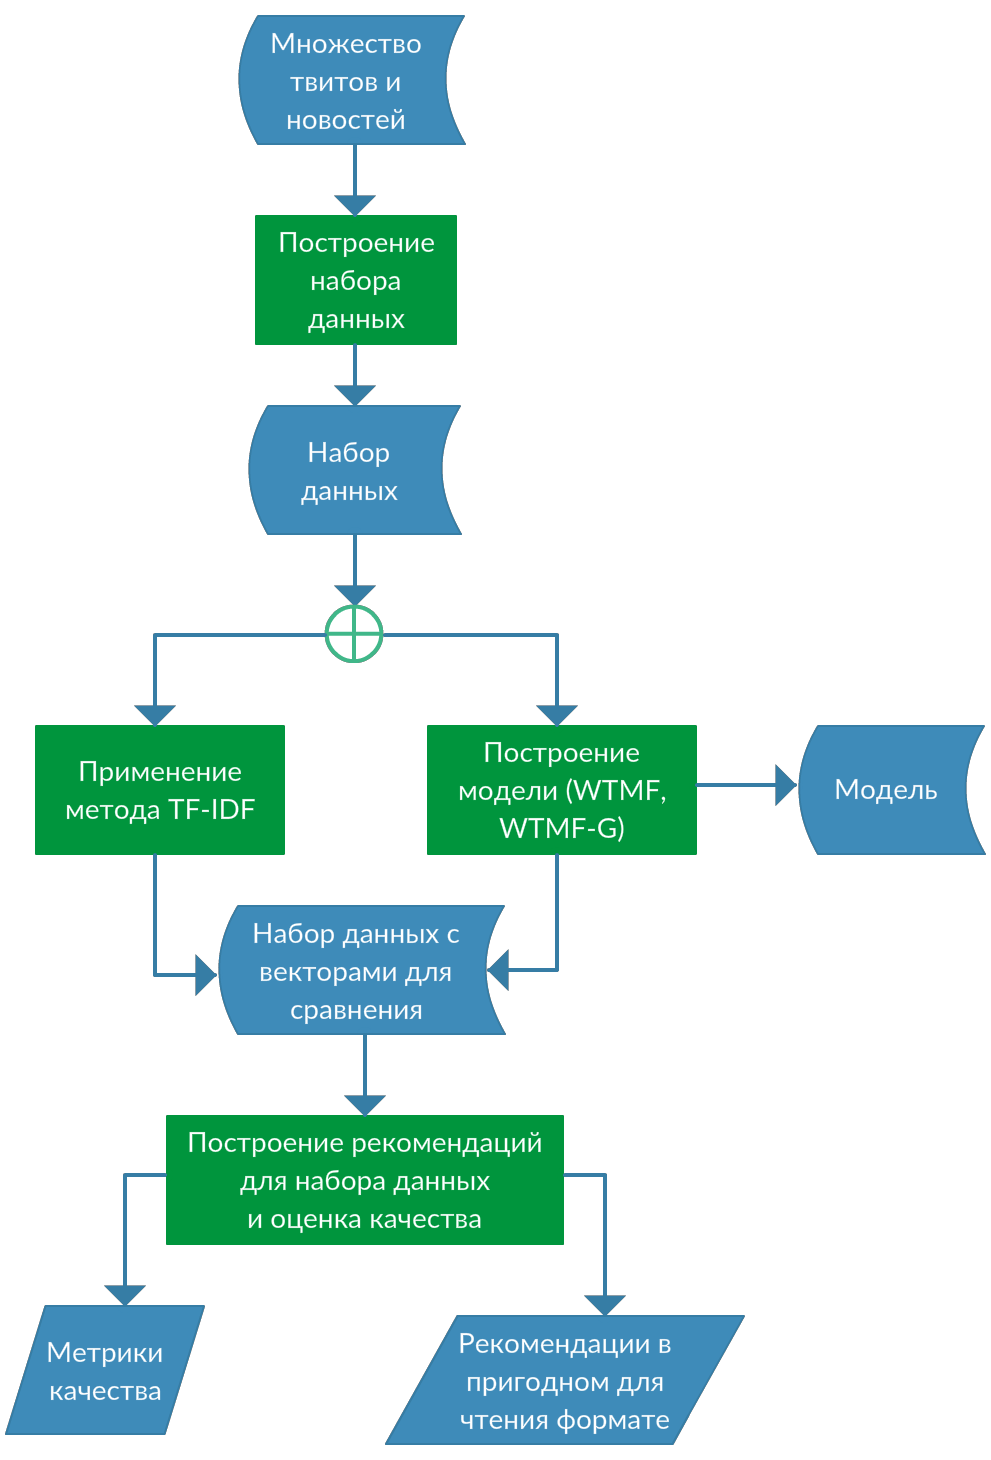
\includegraphics[scale=0.32]{twnews_flowchart_1.png}
            \caption{Блок-схема процесса оценки качества используемых методов}
            \label{pic:twnews_flowchart_1}
    \end{figure}

    На основе построенных рекомендаций можно как произвести оценку качества ранее использованного метода, так и получить их в виде текстового файла,
    который содержит информацию в пригодном для чтения формате.
    Оценка качества использованного метода производится при условии построения рекомендаций для набора данных.
    Процесс оценки качества различных методов рекомендаций, а также получение рекомендаций для твитов из набора данных изображён на рисунке~\ref{pic:twnews_flowchart_1}.

    Дополнительным результатом изображённого на рисунке~\ref{pic:twnews_flowchart_1} процесса является построенная модель (для методов WTMF и WTMF-G), которую можно применить на произвольное множество твитов. Процесс получения рекомендаций для произвольных твитов изображён на рисунке~~\ref{pic:twnews_flowchart_2}.
    
    \begin{figure}[h!]
            \center
            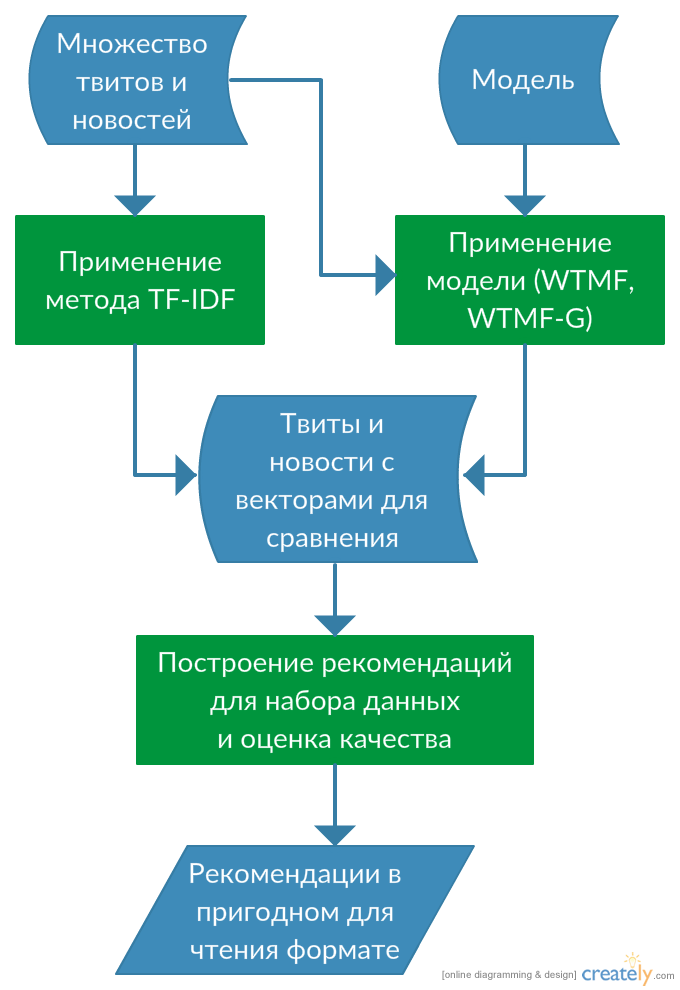
\includegraphics[scale=0.32]{twnews_flowchart_2.png}
            \caption{Блок-схема процесса получения рекомендаций для различных методов}
            \label{pic:twnews_flowchart_2}
    \end{figure}

    %\textcolor{red}{заключительный абзац}

    




    \subsection{Nature Language Processing}
    Всё что связано с обработкой текста

    \subsubsection{Лемматизация}
    \label{subsubsec:lemma}
        что это

        как используется

        https://pythonprogramming.net/stop-words-nltk-tutorial/?completed=/tokenizing-words-sentences-nltk-tutorial/
    \subsubsection{Извлечение имён собственных}
        что это

        Обзор подходов

        объяснение используемого

    \subsection{Метод WTMF}
    Модель для метода WTMF построена на основе мнзаранее подготовленного набора данных.
    В контексте работы набор данных состоит из множества новостей и твитов, из которых в процессе работы извлекается набор текстов
    ~(для твита~---~текст твита, для новости~---~конкатенация заголовка и краткого изложения статьи).

    По множеству текстов, которые получены из набора данных, построена модель, пригодная для сериализации, состоящая из матрицы $P$
    ~(здесь и далее используются обозначения введённые в главе \ref{subsubsec:wtmf}).
    Построение модели зависит от четырёх констант:
    \begin{enumerate}
        \item $K$~---~размерность вектора, по которому производится сравнение~
        (если TF-IDF матрица $X$ была размера $M \times N$, то по завершении работы алгоритма будут получены две матрицы $P$ размера $K \times M$ и $Q$ размера $K \times N$);
        \item $I$~---~число итераций алгоритма построения модели;
        \item $w_M$~---~коэффициент, задающий вес негативного сигнала при построении матрицы весов $W$;
        \item $\lambda$~---~регуляризирующий член.
    \end{enumerate}

    Применение полученной модели на множество твитов представляет собой следующий процесс:
    сначала строится TF-IDF матрица $X$ для новостей из набора данных и множества твитов, затем на основе новой матрицы $X$ строится весовая матрица $W$,
    и наконец на основе построенных матриц $X$ и $W$ и посчитанной на этапе обучения матрицы $P$ выполняется половина итерации алгоритма обучения,
    а именно получение матрицы $Q$ по матрице $P$:
    $$Q_{\cdot, j} = (P W'_j P^T + \lambda I)^{-1} P W'_j X_{j,\cdot}.$$
    В результате получаем вектора для сравнения твитов из заданного множества.
    \subsection{Метод WTMF-G}
    Построение модели для метода WTMF-G основывается на построение модели метода WTMF.
    Набор данных состоит из множества новостей и твитов и связей вида текст-текст, из которых, в процессе работы извлекается набор текстов.
    ~(для твита~---~текст твита, для новости~---~конкатенация заголовка и краткого изложения статьи).

    По множеству текстов, которые получены из набора данных, построена пригодная для сериализации модель, представляющая собой матрицу $P$.
    Построение модели зависит от четырёх констант:
    \begin{enumerate}
        \item $K$~---~размерность вектора, по которому производится сравнение~
        (если TF-IDF матрица $X$ была размера $M \times N$, то по завершении работы алгоритма будут получены две матрицы $P$ размера $K \times M$ и $Q$ размера $K \times N$);
        \item $I$~---~число итераций алгоритма построения модели;
        \item $w_M$~---~коэффициент, задающий вес негативного сигнала при построении матрицы весов $W$;
        \item $\delta$~---~коэффициент, задающий степень влияния связей вида текст-текст.
    \end{enumerate}

    Применение полученной модели на множество твитов производится аналогично применению модели для метода WTMF за исключением двух моментов:
    во-первых, необходимо на основе новостей из набора данных и множества твитов перестроить связи текст-текст, во-вторых получение матрицы $Q$ происходит по следующей формуле:
    $$Q_{\cdot, j} = (P W'_j P^T + \lambda I + \delta  L_j^2 Q_{\cdot,n(j)} diag(L^2_{n(j)})Q_{\cdot,n(j)}^T)^{-1}   (P W'_j X_{j,\cdot} + \delta  L_j Q_{\cdot,n(j)} L_{n(j)}).$$
    В результате получаем вектора для сравнения твитов из заданного множества.
    
\subsection{Эффективная работа с матрицами}
    Построение и применение моделей WTMF и WTMF-G требует большого количества операций над матрицами, что на практике занимает продолжительное время.
    Поэтому задача по повышению эффективности работы с матрицами актуальна.

    Для эффективной работы с матрицами используются программные библиотеки для языка Python numpy и
    scipy~(базируется на библиотеке numpy и расширяет её функционал).

    Оптимизируется формула получения строк матрицы $P$, используемая при построении моделей WTMF и WTMF-G.
    На каждой итерации построения модели происходит многократное выполнение формулы (количество выполнений порядка $10^4$, зависит от размера корпуса):
    $$P_{i, \cdot} = (Q W'_i Q^T + \lambda I)^{-1} Q W'_i X_{i,\cdot}^T.$$

    В начале была написана наивная реализация алгоритма, которая показала производительность, не приемлемую в рамках решения задачи.
    Затем наивная реализация оптимизировалась следующим образом:
    \begin{enumerate}
        \item переход к перемножению матриц с использованием высокопроизводительной библиотеки для языка С OpenBlass~(в библиотеке numpy существует возможность перейти к использованию для работы с матрицами некоторых библиотек, написанных на языке С~\cite{blas_installation});
        \item сохранение в отдельной переменной переиспользуемых результатов вычислений над матрицами;
        \item переписывание кода для работы с разреженными матрицами;
        \item удаление лишних приведений матриц к формату python list и обратно.
    \end{enumerate}
    Результаты оптимизации приведены в таблице~\ref{tabular:matrix_optimization}.

    \begin{table}[ht!]
        %\small
        \caption{Оптимизация работы с матрицами\bigskip}
        \centering

        \label{tabular:matrix_optimization}
        \begin{tabular}{|p{5cm}|c|c|}
            \hline
            \bf{\specialcell{Добавленная \\ оптимизация}} &
            \bf{\specialcell{Время за \\ 100 итераций~(c)}} &
            \bf{\specialcell{Прирост \\ производительности \\ (раз) }} \\ \hline

            Наивная реализация & 205 & 1 \\ \hline
            Перемножение с помощью OpenBlass & 55 & 3.73 \\ \hline
            Переиспользование результатов & 15.15 & 3.63 \\ \hline
            Работа с разреженными матрицами & 0.75 & 20.2 \\ \hline
            Сокращение количества приведений типов & 0.63 & 1.21 \\ \hline
        \end{tabular}
    \end{table}
    Получили, что оптимизированное решение работает в 325 раз быстрее наивной реализации.
    Дальнейшая оптимизация не производилась, так как получено решение работающее за приемлемое время.
%    Дополнительную оптимизацию можно произвести с помощью использования библиотек для работы с матрицами, использующих видеокарт
%
%
%
%    идеи по дальнейшей оптимизации: CUDA

 \clearpage
    \section{Руководство пользователя}
\label{sec:documentation}
    Программный комплекс состоит из двух приложений, каждое из которых устанавливается и используется в отдельности.
    \begin{itemize}
        \item twnews\_consumer~---~приложение, предназначенное для того, чтобы получать твиты с твиттера и новости с rss каналов.
        \item twnews~---~приложение, позволяющее по твитам и новостям, произвести все необходимые для автоматического построения рекомендций
        преобразования данных, построить рекомендации и оценить полученный результат.
    \end{itemize}

    Оба пакета ориентированы на работу в операционных системах семейства linux.
    Для начала работы необходимо получить содержимое git-репозитория: https://github.com/art-vybor/twnews.git, в котором расположены исходный код обоих приложений.
    Если установлен пакет git, то получение git-репозитория происходит с помощью следующей команды:
    \begin{lstlisting}
$ git clone https://github.com/art-vybor/twnews.git
    \end{lstlisting}
    Для сборки приложений необходимо иметь установленный менеджер пакетов языка Python~---~pip. С помощью него необходимо установить Python библиотеку setuptools:
    \begin{lstlisting}
$ pip install setuptools
    \end{lstlisting}

    Отдельно стоит отметить, что для корректной работы пакетов twnews и twnews\_consumer, все директории, указываемые в конфигурации пакетов должны быть созданы заранее.

    \subsection{Пакет twnews\_consumer}
    Исходный код приложения twnews\_consumer расположен в папке \lstinline{consumer} в корне репозитория.
    Приложение позволяет выкачивать и сохранять твиты и новости в формате, удобном для дальнейшей работы пакета twnews.

    \subsubsection{Конфигурирование}
        Конфигурирование пакета twnews\_consumer производится в файле \lstinline{twnews_consumer/defaults.py}.
        После изменения параметров, необходимо переустановить пакет.
        Описание задаваемых параметров находится в таблице~\ref{tabular:consumer_config}.

        \begin{table}[h!]
            \small
            \caption{Описание конфигурации пакета twnews\_consumer \bigskip}
            \center

            %\begin{sideways}
            \label{tabular:consumer_config}
            %\begin{tabular}{|m{0.18cm}|m{0.18cm}|m{0.18cm}|@{}m{0pt}@{}}
            \begin{tabular}{|c|c|m{5cm}|}
                \hline
                \bf{Имя параметра} & \bf{Пример значения} & \bf{Описание} \\ \hline

                LOG\_FILE & \begin{lstlisting}[basicstyle=\small]
'/var/log/twnews_consumer.log'
                \end{lstlisting} & Путь до файла с логом \\ \hline

                LOG\_LEVEL & \begin{lstlisting}[basicstyle=\small]
logging.INFO
                \end{lstlisting} & Уровень подробности лога \\ \hline

                TWNEWS\_DATA\_PATH & \begin{lstlisting}[basicstyle=\small]
'/home/user/twnews_data/'
                \end{lstlisting} & Путь до директории, в которую будут сохранены данные \\ \hline

                RSS\_FEEDS &
                \begin{lstlisting}[basicstyle=\small]
{
'lenta': {'rss_url':
'http://lenta.ru/rss'},
'rt': {'rss_url':
'https://russian.rt.com/rss'},
}
                \end{lstlisting} & Новостные источники, которые требуется выкачать \\ \hline

                TWEETS\_LANGUAGES & \begin{lstlisting}[basicstyle=\small]
['ru']
                \end{lstlisting} & Список языков, твиты с использованием которых выкачиваются из твиттера \\ \hline
            \end{tabular}
            %\end{sideways}
        \end{table}

    \subsubsection{Установка}
        Для установки приложения, необходимо зайти в папку \lstinline{consumer} с исходным кодом пакет twnews\_consumer, находящуюся в корне репозитория, и выполнить команду:

        \begin{lstlisting}
$ make install
        \end{lstlisting}
        Во время установки, с целью распаковки секретного ключа, необходимого для работы с API твиттера, требуется ввести секретный пароль.

    \subsubsection{Использование}
        Результатом работы пакета является множество новостей и твитов, выкаченных за время работы программы.
        Для новостей сохраняются заголовок, краткое описание, ссылка на новость, время публикации и имя ресурса, на котором новость была опубликована.
        Для твитов сохраняются текст, численный уникальный идентификатор ,время публикации, информацию о хэштегах и ссылках и является ли он ретвитом.

        Приложение обладает интерфейсом командной строки.
        Для старта скачивания новостей, необходимо запустить команду:
        \begin{lstlisting}
$ twnews_consumer download --news
        \end{lstlisting}
        Для старта скачивания сообщения твиттера, необходимо запустить команду:
        \begin{lstlisting}
$ twnews_consumer download --tweets
        \end{lstlisting}
        Для завершения скачивания, необходимо использовать сочетание клавиш <<Ctrl-C>>.
        Приложение обработает прерывание и корректно завершится.

        Приложение записывает вспомогательную информацию о своём статусе и обработанных ошибках в файл лога.
        Поэтому из файла лога можно узнать актуальную информацию о работе приложения. Пример:
        \begin{lstlisting}
$ tail -f  /var/log/twnews_consumer.log
2016-04-05 11:37:14: RSS> Start consume rss feeds
2016-04-05 11:37:17: TWITTER> Starting write to /mnt/yandex.disk/twnews_data/logs/tweets.shelve
2016-04-05 11:37:17: TWITTER> Starting to consume twitter
2016-04-05 12:33:32: TWITTER> ('Connection broken: IncompleteRead(0 bytes read, 512 more expected)', IncompleteRead(0 bytes read, 512 more expected))
        \end{lstlisting}

        Приложение twnews\_consumer устойчиво к ошибкам, возникающим при получении новостей и твитов,
        востановление работы заключается в перезапуске скачивания информации.
        Ввиду этого приложение реализует скачивание данных согласно семантики \textit{at-most-once}~---~
        гарантируется отсутствие дублей, но допускается потеря данных.
    \subsection{Пакет twnews}
    Пакет twnews располагается в папке \lstinline{core} в корне репозитория.
    Приложение позволяет обрабатывать данные полученные с помощью консьюмера с целью автоматического установления связей
    между твитами и новостными статьями и оценки качества полученного решения.

    \subsubsection{Конфигурирование}
        Конфигурирование пакета twnews производится в файле \lstinline{twnews/defaults.py}.
        После изменения параметров, необходимо переустановить пакет.
        Описание задаваемых параметров находится в таблице~\ref{tabular:core_config}.
        \begin{table}[h!]
            \small
            \caption{Описание конфигурации пакета twnews \bigskip}
            \center

            \label{tabular:core_config}
            \begin{tabular}{|c|c|m{5cm}|}
                \hline
                \bf{Имя параметра} & \bf{Пример значения} & \bf{Описание} \\ \hline

                LOG\_FILE & \begin{lstlisting}[basicstyle=\small]
'/var/log/twnews.log'
                \end{lstlisting} & Путь до файла с логом \\ \hline

                LOG\_LEVEL & \begin{lstlisting}[basicstyle=\small]
logging.INFO
                \end{lstlisting} & Уровень подробности лога \\ \hline

                TWNEWS\_DATA\_PATH & \begin{lstlisting}[basicstyle=\small]
'/home/user/twnews_data/'
                \end{lstlisting} & Путь до директории, в которую были скачены данные приложением twnews\_consumer \\ \hline

                DATASET\_FRACTION & \begin{lstlisting}[basicstyle=\small]
1.0
\end{lstlisting} & Часть множества скаченных твитов на основе которых происходит построение набора данных \\ \hline

                TMP\_FILE\_DIRECTORY & \begin{lstlisting}[basicstyle=\small]
'/tmp/twnews/'
                \end{lstlisting} & Путь до директории в которую будут сохранены временные данные \\ \hline

                 DEFAULT\_WTMF\_OPTIONS & \begin{lstlisting}[basicstyle=\small]
{
    'DIM': 90,
    'WM': 0.95,
    'ITERATIONS': 1,
    'LAMBDA': 1.95
}
                \end{lstlisting} & Настройки метода WTMF \\ \hline

                 DEFAULT\_WTMFG\_OPTIONS & \begin{lstlisting}[basicstyle=\small]
{
    'DIM': 220,
    'WM': 5,
    'ITERATIONS': 1,
    'DELTA': 0.06,
    'LAMBDA': 6
}
                \end{lstlisting} & Настройки метода WTMF-G \\ \hline

            \end{tabular}
        \end{table}

    \subsubsection{Установка}
        Для установки приложения, необходимо зайти в папку \lstinline{core} с исходным кодом пакет twnews, находящуюся в корне репозитория, и выполнить команду:
        \begin{lstlisting}
$ make install
        \end{lstlisting}
        Для повышения производительности рекомендуется вручную собрать пакет numpy с использованием низкоуровневой математической библиотеки OpenBLAS~\cite{blas_installation}.

    \subsubsection{Использование}
        Финальным результатом работы приложения является получение рекомендаций для произвольных твитов.
        Построение рекомендаций происходит в несколько стадий~(каждая стадия представляет собой отдельный вызов приложения),
        количество стадий различается для различных методов рекомендаций.

        Приложение обладает интерфейсом командной строки.
        Для удобства использования функционал приложения разбивается на набор независимых друг от друга точек входа,
        каждая из которых представляет интерфейс для выполнения одной из стадий работы построения рекомендаций.
        Список всех точек входа представлен в таблице~\ref{tabular:entry_point}.

         \begin{table}[h!]
            \small
            \caption{Описание точек входа пакета twnews \bigskip}
            \center

            \label{tabular:entry_point}
            \begin{tabular}{|c|c|m{7cm}|}
                \hline
                \bf{Название точки входа} & \bf{Пример команды запуска} & \bf{Описание} \\ \hline
                tweets\_sample & twnews tweets\_sample & Получение случайного набора твитов из собранных данных \\ \hline
                resolver & twnews resolver & Расшифровка сокращённых ссылок \\ \hline
                build\_dataset & twnews build\_dataset & Автоматическое построение набора данных \\ \hline
                train & twnews train & Построение модели для методов WTMF и WTMF-G \\ \hline
                apply & twnews apply & Применение модели для методов WTMF и WTMF-G \\ \hline
                tfidf\_dataset & twnews tfidf\_dataset & Применение метода TF-IDF на набор данных \\ \hline
                tfidf\_tweets & twnews tfidf\_tweets & Применение метода TF-IDF на произвольные твиты\\ \hline
                recommend\_dataset & twnews recommend\_dataset & Построение и оценка качества рекомендаций для набора данных \\ \hline
                recommend\_tweets & twnews recommend\_tweets & Построение рекомендаций для произвольных твитов \\ \hline
            \end{tabular}
        \end{table}
        Далее приводится более детальное описание каждой точки входа. Для каждой точки входа в качестве примера использования
        приводится две команды командной строки: результат вызова автоматически порождаемой приложением справочной информации и пример вызова точки входа.

        %
        % tweets_sample
        %

        Точка входа tweets\_sample позволяет получить случайный набор твитов из собранных данных. Параметризуется двумя необязательными параметрами
        length~---~задаёт количество твитов в результате, и tweets~---~определяет полное имя создаваемого файла, который содержит список твитов.
        Пример использования:
        \begin{lstlisting}
$ twnews tweets_sample -h
usage: twnews tweets_sample [-h] [--length LENGTH] [--tweets TWEETS]

optional arguments:
  -h, --help       show this help message and exit
  --length LENGTH  num of tweets in sample (default: 1000)
  --tweets TWEETS  tweets sample filepath (default:
                   /home/avybornov/tmp/tweets_sample)

$ twnews tweets_sample
get sample of random tweets
sample generated and saved at /home/avybornov/tmp/tweets_sample
        \end{lstlisting}

        %
        % build_dataset
        %

        Точка входа build\_dataset позволяет автоматически построить набор данных. Параметризуется двумя необязательными параметрами
        unique\_words~---~задаёт процент уникальных слов в твите для пар твит-новость, и dataset~---~задаёт полное имя создаваемого файла, который содержит набор данных;
        Пример использования:
        \begin{lstlisting}
$ twnews build_dataset -h
usage: twnews build_dataset [-h] [--unique_words UNIQUE_WORDS]
                            [--dataset DATASET]

optional arguments:
  -h, --help            show this help message and exit
  --unique_words UNIQUE_WORDS
                        percent of unique words in tweet by corresponding news
                        (default: 0.0)
  --dataset DATASET     dataset filepath (default:
                        /home/avybornov/tmp/dataset)

$ twnews build_dataset
building automatic dataset
dataset builded and saved at /home/avybornov/tmp/dataset
        \end{lstlisting}

        %
        % resolver
        %

        Точка входа resolver позволяет расшифровать все сокращённые ссылки, используемые в скаченном приложением twnews\_consumer множестве данных~(параметр resolve).
        Отображение коротких ссылок в расшифрованные хранится отдельным файлом и в дальнешем используется при построении набора данных.
        Также точка входа resolver позволяет получить статистику по все расшифрованным ссылкам~(параметр analyze).
        Пример использования:
        \begin{lstlisting}
$ twnews resolver -h
usage: twnews resolver [-h] (--resolve | --analyze)

optional arguments:
  -h, --help  show this help message and exit
  --resolve   resolve urls from all tweets (default: False)
  --analyze   print stats of resolved urls (default: False)

$ twnews resolver resolve
        \end{lstlisting}

        %
        % train
        %

        Точка входа train позволяет построить модели для методов WTMF и WTMF-G. Каждый метод параметризуется тремя необязательными параметрами:
        dataset~---~полное имя файла, содержащего набора данных, model\_dir~---~директория в которую будет сохранён файл модели,
        dataset\_applied~---~полное имя файла, в который будут записаны новости и твиты из набора данных с векторами для сравнения.
        Пример использования:
        \begin{lstlisting}
$ twnews train -h
usage: twnews train [-h] (--wtmf | --wtmf_g) [--dataset DATASET]
                    [--model_dir MODEL_DIR]
                    [--dataset_applied DATASET_APPLIED]

optional arguments:
  -h, --help            show this help message and exit
  --wtmf                wtmf method (default: False)
  --wtmf_g              wtmf_g method (default: False)
  --dataset DATASET     dataset filepath (default:
                        /home/avybornov/tmp/dataset)
  --model_dir MODEL_DIR
                        name of directory to save model (default:
                        /home/avybornov/tmp)
  --dataset_applied DATASET_APPLIED
                        dataset_applied filepath (default:
                        /home/avybornov/tmp/dataset_applied)

$ twnews train --wtmf
train model
apply model to dataset
model dumped to /home/avybornov/tmp/WTMF_(dataset_auto_0.0)_90_1_1.95_0.95
applied dataset saved: /home/avybornov/tmp/dataset_applied


        \end{lstlisting}

        %
        % apply
        %

        Точка входа apply позволяет применить ранее построенные модели для методов WTMF и WTMF-G на набор твитов.
        Каждый метод параметризуется тремя параметрами: model~---~полное имя файла, содержащего модель,
        tweets~---~полное имя файла с множеством твитов, который был построен с использованием точки входа tweets\_sample,
        tweets\_applied~---~полное имя файла, в который будут записаны полученнные твиты с векторами для сравнения.
        Пример использования:
        \begin{lstlisting}
$ twnews apply -h
usage: twnews apply [-h] (--wtmf | --wtmf_g) [--model MODEL] [--tweets TWEETS]
                    [--tweets_applied TWEETS_APPLIED]

optional arguments:
  -h, --help            show this help message and exit
  --wtmf                wtmf method (default: False)
  --wtmf_g              wtmf_g method (default: False)
  --model MODEL         model filepath (default: /home/avybornov/tmp/WTMF_(dat
                        aset_auto_0.0)_90_1_1.95_0.95)
  --tweets TWEETS       tweets sample filepath (default:
                        /home/avybornov/tmp/tweets_sample)
  --tweets_applied TWEETS_APPLIED
                        tweets_applied filepath (default:
                        /home/avybornov/tmp/tweets_applied)

$ twnews apply --wtmf --model /home/avybornov/tmp/WTMF_\(dataset_auto_0.0\)_90_1_1.95_0.95
apply model
tweets applied and stored at /home/avybornov/tmp/tweets_applied

        \end{lstlisting}

        %
        % tfidf_dataset
        %

        Точка входа tfidf\_dataset позволяет применить метод TFIDF для нахождения векторов сравнения для новостей и твитов из набора данных.
        Параметризуется двумя параметрами
        dataset~---~полное имя файла, содержащего набор данных,
        dataset\_applied~---~полное имя файла, в который будут записаны новости и твиты из набора данных с векторами для сравнения.
        Пример использования:
        \begin{lstlisting}
twnews tfidf_dataset -h
usage: twnews tfidf_dataset [-h] [--dataset DATASET]
                            [--dataset_applied DATASET_APPLIED]

optional arguments:
  -h, --help            show this help message and exit
  --dataset DATASET     dataset filepath (default:
                        /home/avybornov/tmp/dataset)
  --dataset_applied DATASET_APPLIED
                        dataset_applied filepath (default:
                        /home/avybornov/tmp/dataset_applied)

$ twnews tfidf_dataset
apply tfidf to dataset
dataset applied and stored at /home/avybornov/tmp/dataset_applied
        \end{lstlisting}

        %
        % tfidf_tweets
        %

        Точка входа tfidf\_tweets позволяет применить метод TFIDF для нахождения векторов сравнения для набора данных~(как в случае с точкой входа tfidf\_dataset).
        Параметризуется четырьмы параметрами
        dataset~---~полное имя файла, содержащего набор данных,
        dataset\_applied~---~полное имя файла, в который будут записаны новости и твиты из набора данных с векторами для сравнения,
        tweets~---~полное имя файла с множеством твитов, который был построен с использованием точки входа tweets\_sample,
        tweets\_applied~---~полное имя файла, в который будут записаны полученнные твиты с векторами для сравнения.
        Пример использования:
        \begin{lstlisting}
$ twnews tfidf_tweets -h
usage: twnews tfidf_tweets [-h] [--dataset DATASET]
                           [--dataset_applied DATASET_APPLIED]
                           [--tweets TWEETS] [--tweets_applied TWEETS_APPLIED]

optional arguments:
  -h, --help            show this help message and exit
  --dataset DATASET     dataset filepath (default:
                        /home/avybornov/tmp/dataset)
  --dataset_applied DATASET_APPLIED
                        dataset_applied filepath (default:
                        /home/avybornov/tmp/dataset_applied)
  --tweets TWEETS       tweets sample filepath (default:
                        /home/avybornov/tmp/tweets_sample)
  --tweets_applied TWEETS_APPLIED
                        tweets_applied filepath (default:
                        /home/avybornov/tmp/tweets_applied)

$ twnews tfidf_tweets
apply tfidf to dataset
dataset applied and stored at /home/avybornov/tmp/dataset_applied
apply tfidf to tweets
tweets applied and stored at /home/avybornov/tmp/tweets_applied
        \end{lstlisting}


        %
        % recommend_dataset
        %

        Точка входа recommend\_dataset позволяет построить рекомендации по набору новостей и твитов из набора данных с векторами для сравнения
        и получить метрики качества построенных рекомендаций.
        Параметризуется двумя параметрами:
        dataset\_applied~---~название используемого набора данных с векторами для сравнения;
        dump~---~имя файла в который будут сохранены полученные рекомендации.
        Пример использования:
        \begin{lstlisting}
$ twnews recommend_dataset -h
usage: twnews recommend_dataset [-h] [--dataset_applied DATASET_APPLIED]
                                [--dump DUMP]

optional arguments:
  -h, --help            show this help message and exit
  --dataset_applied DATASET_APPLIED
                        dataset_applied filepath (default:
                        /home/avybornov/tmp/dataset_applied)
  --dump DUMP           recommendation dump filepath (default:
                        /home/avybornov/tmp/reccommendation_dump)
$ twnews recommend_dataset
build recommendation
recommendation result evaluation
RR = 0.908454481596
TOP1 = 0.869796484736
TOP3 = 0.940564292322
recommendation dumped to /home/avybornov/tmp/reccommendation_dump
        \end{lstlisting}

        %
        % recommend_tweets
        %

        Точка входа recommend\_tweets позволяет построить рекомендации для произвольных твитов с векторами для сравнения.
        Ввиду большого количества "мусорных" твитов, то есть тех, которые не имеют отношения к новостям, результаты рекомендаций
        для произвольных твитов фильтруются, а именно, оставляются только те твиты, для которых нашлась новость похожая на них
        с коэффициентом схожести превышающем 0.4~(значение было подобрано эмпирически).
        Параметризуется тремя параметрами
        dataset\_applied~---~название используемого набора данных с векторами для сравнения;
        tweets\_applied~---~название файла с набором твитов c векторами для сравнения;
        dump~---~имя файла в который будут сохранены полученные рекомендации.
        Пример использования:
        \begin{lstlisting}
$ twnews recommend_tweets -h
usage: twnews recommend_tweets [-h] [--dataset_applied DATASET_APPLIED]
                               [--tweets_applied TWEETS_APPLIED] [--dump DUMP]

optional arguments:
  -h, --help            show this help message and exit
  --dataset_applied DATASET_APPLIED
                        dataset_applied filepath (default:
                        /home/avybornov/tmp/dataset_applied)
  --tweets_applied TWEETS_APPLIED
                        tweets_applied filepath (default:
                        /home/avybornov/tmp/tweets_applied)
  --dump DUMP           recommendation dump filepath (default:
                        /home/avybornov/tmp/reccommendation_dump)
$ twnews recommend_tweets
recommendation dumped to /home/avybornov/tmp/reccommendation_dump

        \end{lstlisting}


        Приложение записывает вспомогательную информацию о своём статусе и обработанных ошибках в файл лога.
        Поэтому из файла лога можно узнать актуальную информацию о работе приложения. Пример:
        \begin{lstlisting}
$ tail -f /var/log/twnews.log
INFO:root:70.00% of iteration finished
INFO:root:80.00% of iteration finished
INFO:root:90.00% of iteration finished
INFO:root:100% of iteration finished
INFO:root:recommendation dumped to /home/avybornov/tmp/reccommendation_dump
        \end{lstlisting} \clearpage
    \section{Эсперименты}
    Главное целью проведения экспериментов является сравнение двух реализованных методов автоматического установления связей между твитами и новостными статьями:
    метод основанный на частотности употребления слов и WTMF-G.
    Для исследования влияния на качество добавления информации о взаимосвязях вида текст-текст также производится сравнительное тестирование методов WTMF и WTMF-G.

    Ввиду малого числа твитов в наборах данных тестирование производится на тех же выборках, на которых производится обучение.

    \subsection{Оценка качества}
    формулирование того как переходим к рекомендациям и что вообще в них меряем

    \subsubsection{RR}
        описание метрики
    \subsubsection{TOP10}
        описание метрики
    \subsubsection{ATOP}
        описание метрики и обоснование почему она не очень

        Используем метрику $ATOP$ (метрика подробно описана в \cite{steck_recommender}).
        Рассмотрим что означает эта метрика в применении к нашей задаче (я немного модифицировал метрику, для более простого описания, полученная метрика полностью совпадает с описанной метрикой).
        Пусть $T$ - это множество твитов, $N \in \mathbb{N}$ - размер рассматриваемого топа новостей для твита (могут быть все новости вообще), $k < N \in \mathbb{N}$.
        $TOPK_t(k) = 1$, если твит $t \in T$ соответствует хотя бы одной новости в top-k результатов, иначе $TOPK_t(k) = 0$
        $$TOPK(k) = \dfrac {\sum_{t \in T} TOPK_t(k)} {|T|},$$
        $$ATOP = \dfrac{\sum_{k=1}^N TOPK_t(k)}{N} = \dfrac{1}{|T| * N} \sum_{k=\overline{1,N}, ~t \in T} TOPK_t(k).$$

        Значения метрики $ATOP$ лежат на отрезке $[0,1]$. Чем ближе $ATOP$ к $1$ тем лучше.
    \subsection{Метод WTMF}
    Модель для метода WTMF построена на основе мнзаранее подготовленного набора данных.
    В контексте работы набор данных состоит из множества новостей и твитов, из которых в процессе работы извлекается набор текстов
    ~(для твита~---~текст твита, для новости~---~конкатенация заголовка и краткого изложения статьи).

    По множеству текстов, которые получены из набора данных, построена модель, пригодная для сериализации, состоящая из матрицы $P$
    ~(здесь и далее используются обозначения введённые в главе \ref{subsubsec:wtmf}).
    Построение модели зависит от четырёх констант:
    \begin{enumerate}
        \item $K$~---~размерность вектора, по которому производится сравнение~
        (если TF-IDF матрица $X$ была размера $M \times N$, то по завершении работы алгоритма будут получены две матрицы $P$ размера $K \times M$ и $Q$ размера $K \times N$);
        \item $I$~---~число итераций алгоритма построения модели;
        \item $w_M$~---~коэффициент, задающий вес негативного сигнала при построении матрицы весов $W$;
        \item $\lambda$~---~регуляризирующий член.
    \end{enumerate}

    Применение полученной модели на множество твитов представляет собой следующий процесс:
    сначала строится TF-IDF матрица $X$ для новостей из набора данных и множества твитов, затем на основе новой матрицы $X$ строится весовая матрица $W$,
    и наконец на основе построенных матриц $X$ и $W$ и посчитанной на этапе обучения матрицы $P$ выполняется половина итерации алгоритма обучения,
    а именно получение матрицы $Q$ по матрице $P$:
    $$Q_{\cdot, j} = (P W'_j P^T + \lambda I)^{-1} P W'_j X_{j,\cdot}.$$
    В результате получаем вектора для сравнения твитов из заданного множества.
    \subsection{Оптимизация качества WTMF-G, путём варьирования параметров}
    Оптимизация параметров модели для метода WTMF-G будет производится на наборе данных cutted, используя метрику МRR.
    Модель WTMF-G зависит от пяти параметров: $K$, $I$, $\lambda$, $\delta$, $w_m$.
    Параметры $K$ и $I$ влияют на время построения модели, а параметры $\lambda$ и $w_m$ не влияют на время построения модели.

    В качестве начального приближения параметров взяты оптимальные параметры для метода WTMF, а именно $K=90$, $I=1$, $w_m=1.95$,$\lambda=0.95$. В качестве начального приближения параметра $\delta$ берем значение 0.1.

    Сначала оптимизируем параметры, влияющие на регуляризующий член: $\lambda$ и $\delta$,
    Для этого фиксируем остальные параметры: $I=1$, $K=90$, $w_m=1.95$.
    Сначала найдём оптимальный порядок значений начального приближения. Результаты занесены в таблицу~\ref{tabular:wtmfg_test1}.

    \begin{table}[ht!]
        %\small
        \caption{Качество работы алгоритма WMTF-G для различных значений $\lambda$ и $\delta$ при фиксированных значениях $I=1$, $K=90$, $w_m=1.95$. \bigskip}
        \centering

        \label{tabular:wtmfg_test1}
        \begin{tabular}{|c|c|c|c|c|c|} \hline
            $\lambda \backslash \delta$ & \bf{0.001} & \bf{0.01} & \bf{0.1} & \bf{1} & \bf{10}  \\ \hline
            \bf{0.01} & 0.3889 & 0.3842 & 0.3924 & 0.3900 & 0.3895 \\ \hline
            \bf{0.1}  & 0.4895 & 0.4875 & 0.4886 & 0.4850 & 0.4847  \\ \hline
            \bf{1}    & 0.8227 & 0.8256 & 0.8242 & 0.8225 & 0.8212 \\ \hline
            \bf{10}   & 0.8477 & 0.8440 & 0.8496 & 0.8454 & 0.8495 \\ \hline
            \bf{100}  & 0.8294 & 0.8318 & 0.8283 & 0.8240  & 0.8243 \\ \hline
        \end{tabular}
    \end{table}

    Как видно из таблицы~\ref{tabular:wtmfg_test1} порядок параметра $\delta$ оказывает влияние на качество, но достаточно слабое, порядок параметра $\lambda$, напротив очень сильно влияет на получаемое качество.
    Максимальное значение метрики достигнуто при $\lambda=10$ и $\delta=0.1$.
    Для уточнения значения коэффициентов, производится исследование качества работы алгоритма в окрестностях максимального значения метрики.
    Результаты приведены в таблице~\ref{tabular:wtmfg_test2}.

    \begin{table}[ht!]
        %\small
        \caption{Качество работы алгоритма WMTF-G для различных значений $\lambda$ и $\delta$ при фиксированных значениях $I=1$, $K=90$, $w_m=1.95$. \bigskip}
        \centering

        \label{tabular:wtmfg_test2}
        \begin{tabular}{|c|c|c|c|c|c|} \hline
            $\lambda \backslash \delta$ & \bf{0.06} & \bf{0.08} & \bf{0.1} & \bf{0.12} & \bf{0.14}  \\ \hline
            \bf{4}  & 0.8501 & 0.8512 & 0.8489 & 0.8530 & 0.8476  \\ \hline
            \bf{6}  & 0.8589 & 0.8524 & 0.8511 & 0.8580 & 0.8493  \\ \hline
            \bf{8}  & 0.8483 & 0.8528 & 0.8539 & 0.8439 & 0.8498  \\ \hline
            \bf{10} & 0.8504 & 0.8455 & 0.8416 & 0.8453 & 0.8408  \\ \hline
            \bf{12} & 0.8453 & 0.8398 & 0.8472 & 0.8376 & 0.8415  \\ \hline
            \bf{14} & 0.8462 & 0.8456 & 0.8387 & 0.8398 & 0.8377  \\ \hline
        \end{tabular}
    \end{table}

    В таблице~\ref{tabular:wtmfg_test2} получена достаточно однородная картина. Возьмём в качестве оптимального значения коэффициент полученную точку максимум: $\lambda=6$, $\delta=0.06$.

    Рассмотрим влияние параметра $w_m$ и найдём его оптимальное значение. Сначала рассмотрим качество алгоритма для различных порядков $w_m$.
    Результаты занесены в таблицу~\ref{tabular:wtmfg_test3}

    \begin{table}[ht!]
        %\small
        \caption{Качество работы алгоритма WMTF-G для различных значений $w_m$ при фиксированных значениях $I=1$, $K=90$, $\lambda=6$, $\delta=0.6$. \bigskip}
        \centering

        \label{tabular:wtmfg_test3}
        \begin{tabular}{|c|c|c|c|c|c|c|c|c|c|} \hline
            $w_m$ & 0.01 & 0.05 & 0.1 & 0.5 & 1 & 5 & 10 & 50 & 100 \\ \hline
            \bf{MRR} & 0.8283 & 0.8296 & 0.8285 & 0.8359 & 0.8442 & 0.8639 & 0.8391 & 0.6094 & 0.5035 \\ \hline

        \end{tabular}
    \end{table}

    Как видно из таблицы~\ref{tabular:wtmfg_test3} порядок параметра $w_m$ оказывает заметное влияние на качество. При значительном увеличении до $10^2$ качество начинает резко падать.
    Максимальное значение метрики достигнуто при $w_m=5$, уточним полученное значение.
    Для уточнения значения коэффициента $w_m$, производится исследование качества работы алгоритма в окрестностях максимального значения метрики.
    Результаты приведены в таблице~\ref{tabular:wtmfg_test4}.

    \begin{table}[ht!]
        %\small
        \caption{Качество работы алгоритма WMTF-G для различных значений $w_m$ при фиксированных значениях $I=1$, $K=90$, $\lambda=6$, $\delta=0.6$. \bigskip}
        \centering

        \label{tabular:wtmfg_test4}
        \begin{tabular}{|c|c|c|c|c|c|c|c|c|c|c|c|c|} \hline
            $w_m$ & 3.0 & 3.5 & 4.0 & 4.5 & 5.0 & 5.5 & 6.0 & 6.5 & 7.5 \\ \hline
            \bf{MRR} & 0.8592 & 0.8585 & 0.8594 & 0.8603 & 0.8641 & 0.8591 & 0.8586 & 0.8574 & 0.8536 \\ \hline

        \end{tabular}
    \end{table}

    Из таблицы~\ref{tabular:wtmfg_test4} получаем оптимальное значение параметра $w_m=5$.
    Теперь рассмотрим оставшиеся два параметра $K$ и $I$. Качество работы алгоритма WTMF-G для различных значений $K$ и $I$ приведено в таблице~\ref{tabular:wtmfg_test5}.

    \begin{table}[ht!]
        %\small
        \caption{Качество работы алгоритма WMTF-G для различных значений $K$ и $I$ при фиксированных значениях $w\_m=5$, $\lambda=6$, $\delta=0.06$. \bigskip}
        \centering
        \label{tabular:wtmfg_test5}
        \begin{tabular}{|c|c|c|c|c|c|} \hline
            $K \backslash I$ & 1 & 2 & 3 & 4 & 5  \\ \hline
            30 & 0.7529 & 0.7927 & 0.7577 & 0.6736 & 0.5794  \\ \hline
            40 & 0.7992 & 0.8194 & 0.7695 & 0.6813 & 0.5828  \\ \hline
            50 & 0.8269 & 0.8349 & 0.7834 & 0.6830 & 0.5801  \\ \hline
            60 & 0.8419 & 0.8450 & 0.7984 & 0.7056 & 0.6006  \\ \hline
            70 & 0.8557 & 0.8466 & 0.7977 & 0.7036 & 0.6002  \\ \hline
            80 & 0.8614 & 0.8511 & 0.7990 & 0.7032 & 0.5957  \\ \hline
            90 & 0.8606 & 0.8522 & 0.8039 & 0.7088 & 0.6038  \\ \hline
            100 & 0.8606 & 0.8527 & 0.8022 & 0.7089 & 0.6021  \\ \hline
            110 & 0.8686 & 0.8553 & 0.8074 & 0.7123 & 0.6065  \\ \hline
            120 & 0.8693 & 0.8579 & 0.8097 & 0.7174 & 0.6085  \\ \hline
            130 & 0.8725 & 0.8588 & 0.8160 & 0.7264 & 0.6206  \\ \hline
            140 & 0.8740 & 0.8597 & 0.8157 & 0.7248 & 0.6241  \\ \hline
            150 & 0.8763 & 0.8620 & 0.8171 & 0.7263 & 0.6200  \\ \hline
            160 & 0.8740 & 0.8596 & - & - & - \\ \hline
            170 & 0.8768 & 0.8606 & - & - & -  \\ \hline
            180 & 0.8785 & 0.8613 & - & - & -  \\ \hline
            190 & 0.8767 & 0.8616 & - & - & -  \\ \hline
            200 & 0.8769 & 0.8613 & - & - & -  \\ \hline
            210 & 0.8786 & 0.8613 & - & - & -  \\ \hline
            220 & 0.8816 & 0.8632 & - & - & -  \\ \hline
            230 & 0.8814 & 0.8646 & - & - & -  \\ \hline
            240 & 0.8758 & 0.8632 & - & - & -  \\ \hline
        \end{tabular}
    \end{table}

    Как показано в таблице~\ref{tabular:wtmfg_test5}, WTMF-G показывает аналогично методу WTMF поведение при изменении параметров $K$ и $I$, а именно, в среднем с увеличением количества итераций, качество работы алгоритма уменьшается.
    Максимум был достигнут при $K=220$, $I=1$.

    В итоге оптимизации качества рекомендаций на основе алгоритма WMTF-G были получены оптимальные параметры:
    $K=220$, $I=1$, $\delta=0.6$, $\lambda=6$, $w_m=5$.

    \clearpage
    \subsection{Сравнительные результаты}
    Для выявления влияния добавления связей текст-текст на результаты работы метода WMTF-G производится сравнительное тестирование алгоритма WTMF и WTMF-G.
    Результаты тестирования приведены в таблице~\ref{tabular:wtmf_wmtfg}.

    \begin{table}[h!]
    %\small
    \caption{Cравнительное тестирование алгоритмов WTMF и WTMF-G. \bigskip}
    \centering

    \label{tabular:wtmf_wmtfg}
        \begin{tabular}{|c|c|c|c|c|c|c|}
            \hline
            \bf{\multirow{2}{*}{\specialcell{Набор данных}}} &
            \multicolumn{2}{|c|}{\bf{Метрика RR}} &
            \multicolumn{2}{|c|}{\bf{Метрика $TOP_1$}} &
            \multicolumn{2}{|c|}{\bf{Метрика $TOP_3$}} \\ \cline{2-7}
            & \bf{WTMF} & \bf{WTMF-G} & \bf{WTMF} & \bf{WTMF-G} & \bf{WTMF} & \bf{WTMF-G} \\ \hline
            manual & 0.7293 & 0. & 0. & 0. & 0. & 0. \\ \hline
            auto & 0.8640 & 0. & 0. & 0. & 0. & 0. \\ \hline
            total & 0.8196 & 0. & 0. & 0. & 0. & 0. \\ \hline
            cutted & 0.8630 & 0. & 0. & 0. & 0. & 0. \\ \hline
            manual\_nt & 0.6194 & 0. & 0. & 0. & 0. & 0. \\ \hline
            auto\_nt & 0.5297 & 0.5695 & 0. & 0. & 0. & 0. \\ \hline
            total\_nt & 0.5729 & 0. & 0. & 0. & 0. & 0. \\ \hline
            cutted\_nt & 0.6495 & 0. & 0. & 0. & 0. & 0. \\ \hline
        \end{tabular}
    \end{table}
    Как видно из таблицы~\ref{tabular:wtmf_wmtfg} \textcolor{red}{...}

    \textcolor{red}{Сравним метод основанный на частотности употребления слов и WTMF-G.}
    Метод основанный на частотности употребления слов обозначим как TF-IDF.
    Результаты тестирования приведены в таблице~\ref{tabular:tfidf_wmtfg}.

    \begin{table}[ht!]
    %\small
    \caption{Cравнительное тестирование алгоритмов TF-IDF и WTMF-G. \bigskip}
    \centering

    \label{tabular:tfidf_wmtfg}
        \begin{tabular}{|c|c|c|c|c|c|c|}
            \hline
            \bf{\multirow{2}{*}{\specialcell{Набор данных}}} &
            \multicolumn{2}{|c|}{\bf{Метрика RR}} &
            \multicolumn{2}{|c|}{\bf{Метрика $TOP_1$}} &
            \multicolumn{2}{|c|}{\bf{Метрика $TOP_3$}} \\ \cline{2-7}
            & \bf{TF-IDF} & \bf{WTMF-G} & \bf{TF-IDF} & \bf{WTMF-G} & \bf{TF-IDF} & \bf{WTMF-G} \\ \hline
            manual & 0.8336 & 0. & 0. & 0. & 0. & 0. \\ \hline
            auto & 0.8817 & 0. & 0. & 0. & 0. & 0. \\ \hline
            total & 0.8610 & 0. & 0. & 0. & 0. & 0. \\ \hline
            cutted & 0.9075 & 0. & 0. & 0. & 0. & 0. \\ \hline
            manual\_nt & 0.7565 & 0. & 0. & 0. & 0. & 0. \\ \hline
            auto\_nt & 0.6048 & 0.5695 & 0. & 0. & 0. & 0. \\ \hline
            total\_nt & 0.6914 & 0. & 0. & 0. & 0. & 0. \\ \hline
            cutted\_nt & 0.7485 & 0. & 0. & 0. & 0. & 0. \\ \hline
        \end{tabular}
    \end{table}
    Как видно из таблицы~\ref{tabular:tfidf_wmtfg} \textcolor{red}{...}

    объяснение влияния различных датасетов, специфики русского языка и сравнение с результатами статьи.



 \clearpage
    \section{Технико-экономическое обоснование}
    Разработка программного обеспечения~---~достаточно трудоемкий и длительный процесс, требующий выполнения большого числа разнообразных операций.
    Организация и планирование процесса разработки программного продукта или программного комплекса при традиционном методе планирования предусматривает выполнение следующих работ~\cite{economic_smirnov}:
    \begin{itemize}
        \item формирование состава выполняемых работ и группировка их по стадиям разработки;
        \item расчет трудоемкости выполнения работ;
        \item установление профессионального состава и расчет количества исполнителей;
        \item определение продолжительности выполнения отдельных этапов разработки;
        \item построение календарного графика выполнения разработки;
        \item контроль выполнения календарного графика.
    \end{itemize}

    Далее приведен перечень и состав работ при разработке программного средства для автоматического установления связей между сообщениями твиттера и новостными статьями.
    Отметим, что процесс разработки программного продукта характеризуется совместной работой разработчиков постановки задач и разработчиков программного обеспечения.

    Укрупненный состав работ по стадиям разработки программного продукта~\cite{gost_34601}~\cite{economic_sajin}:
    \begin{enumerate}
        \item Техническое задание:
            \begin{itemize}
                \item Постановка задач, выбор критериев эффективности,
                \item Разработка технико-экономического обоснования разработки,
                \item Определение состава пакета прикладных программ, состава и структуры информационной базы,
                \item Выбор языков программирования,
                \item Предварительный выбор методов выполнения работы,
                \item Разработка календарного плана выполнения работ;
            \end{itemize}
        \item Эскизный проект:
            \begin{itemize}
                \item Предварительная разработка структуры входных и выходных данных,
                \item Разработка общего описания алгоритмов реализации решения задач,
                \item Разработка пояснительной записки,
                \item Консультации разработчиков постановки задач,
                \item Согласование и утверждение эскизного проекта;
            \end{itemize}
        \item Технический проект:
            \begin{itemize}
                \item Разработка алгоритмов решения задач,
                \item Разработка пояснительной записки,
                \item Согласование и утверждение технического проекта,
                \item Разработка структуры программы,
                \item Разработка программной документации и передача ее для включения в технический проект,
                \item Уточнение структуры, анализ и определение формы представления входных и выходных данных,
                \item Выбор конфигурации технических средств;
            \end{itemize}
        \item Рабочий проект:
            \begin{itemize}
                \item Комплексная отладка задач и сдача в опытную эксплуатацию,
                \item Разработка проектной документации,
                \item Программирование и отладка программ,
                \item Описание контрольного примера,
                \item Разработка программной документации,
                \item Разработка, согласование программы и методики испытаний,
                \item Предварительное проведение всех видов испытаний;
            \end{itemize}
        \item Внедрение:
            \begin{itemize}
                \item Подготовка и передача программной документации для сопровождения с оформлением соответствующего Акта,
                \item Передача программной продукции в фонд алгоритмов и программ,
                \item Проверка алгоритмов и программ решения задач, корректировка документации после опытной эксплуатации программного продукта;
            \end{itemize}
    \end{enumerate}

    Трудоемкость разработки программной продукции зависит от ряда факторов, основными из которых являются следующие: степень новизны разрабатываемого программного комплекса, сложность алгоритма его функционирования, объем используемой информации, вид ее представления и способ обработки, а также уровень используемого алгоритмического языка программирования.
    Чем выше уровень языка, тем трудоемкость меньше.

    По степени новизны разрабатываемый проект относится к \textit{группе новизны A} – разработка программных комплексов, требующих использования принципиально новых методов их создания, проведения НИР и т.п.

    По степени сложности алгоритма функционирования проект относится к \textit{2 группе сложности} - программная продукция, реализующая учетно-статистические алгоритмы.

    По виду представления исходной информации и способа ее контроля программный продукт относится к \textit{группе 12} - исходная информация представлена в форме документов, имеющих различный формат и структуру и \textit{группе 22} - требуется печать документов одинаковой формы и содержания, вывод массивов данных на машинные носители.

    \subsection{Трудоемкость разработки программной продукции}
    \label{subsec:trud}
        Трудоемкость разработки программной продукции~($\tau_{PP}$) может быть определена как сумма величин трудоемкости выполнения отдельных стадий разработки программного продукта из выражения:
        \begin{equation}
            \tau_{PP} = \tau_{TZ} + \tau_{EP} + \tau_{TP} + \tau_{RP} + \tau_{V},
        \end{equation}
        где $\tau_{TZ}$~---~трудоемкость разработки технического задания на создание программного продукта;
        $\tau_{EP}$~---~трудоемкость разработки эскизного проекта программного продукта;
        $\tau_{TP}$~---~трудоемкость разработки технического проекта программного продукта;
        $\tau_{RP}$~---~трудоемкость разработки рабочего проекта программного продукта;
        $\tau_{V}$~---~трудоемкость внедрения разработанного программного продукта.

        \subsubsection{Трудоемкость разработки технического задания}
            Расчёт трудоёмкости разработки технического задания~($\tau_{PP}$)~[чел.-дни] производится по формуле:
            \begin{equation}
                \tau_{TZ} = T^Z_{RZ} + T^Z_{RP},
            \end{equation}
            где $T^Z_{RZ}$~---~затраты времени разработчика постановки задачи на разработку ТЗ,~[чел.-дни];
            $T^Z_{RP}$~---~затраты времени разработчика программного обеспечения на разработку ТЗ,~[чел.-дни].
            Их значения рассчитываются по формулам:
            \begin{equation}
                T^Z_{RZ} = t_Z  \cdot  K^Z_{RZ},
            \end{equation}
            \begin{equation}
                T^Z_{RP} = t_Z  \cdot  K^Z_{RP},
            \end{equation}
            где $t_Z$~--~норма времени на разработку ТЗ на программный продукт~(зависит от функционального назначения и степени новизны разрабатываемого программного продукта),~[чел.-дни].
            В нашем случае по таблице получаем значение~(группа новизны – А, функциональное назначение – технико-экономическое планирование):
            \begin{equation*}
                t_Z = 79.
            \end{equation*}
            $K^Z_{RZ}$~---~коэффициент, учитывающий удельный вес трудоемкости работ, выполняемых разработчиком постановки задачи на стадии ТЗ.
            В нашем случае~(совместная разработка с разработчиком ПО):
            \begin{equation*}
                K^Z_{RZ} = 0.65.
            \end{equation*}
            $K^Z_{RP}$~---~коэффициент, учитывающий удельный вес трудоемкости работ, выполняемых разработчиком программного обеспечения на стадии ТЗ.
            В нашем случае~(совместная разработка с разработчиком постановки задач):
            \begin{equation*}
                K^Z_{RP} = 0.35.
            \end{equation*}
            Тогда:
            \begin{equation*}
                \tau_{TZ} = 79  \cdot (0.35 + 0.65) = 79.
            \end{equation*}

        \subsubsection{Трудоемкость разработки эскизного проекта}
            Расчёт трудоёмкости разработки эскизного проекта~($\tau_{EP}$)~[чел.-дни] производится по формуле:
            \begin{equation}
                \tau_{EP} = T^E_{RZ} + T^E_{RP},
            \end{equation}
            где $T^E_{RZ}$~---~затраты времени разработчика постановки задачи на разработку эскизного проекта~(ЭП),~[чел.-дни];
            $T^E_{RP}$~---~затраты времени разработчика программного обеспечения на разработку ЭП,~[чел.-дни].
            Их значения рассчитываются по формулам:
            \begin{equation}
                T^E_{RZ} = t_E  \cdot  K^E_{RZ},
            \end{equation}
            \begin{equation}
                T^E_{RP} = t_E  \cdot  K^E_{RP},
            \end{equation}
            где $t_E$~--~норма времени на разработку ЭП на программный продукт~(зависит от функционального назначения и степени новизны разрабатываемого программного продукта),~[чел.-дни].
            В нашем случае по таблице получаем значение~(группа новизны – А, функциональное назначение – технико-экономическое планирование):
            \begin{equation*}
                t_E = 175.
            \end{equation*}
            $K^E_{RZ}$~---~коэффициент, учитывающий удельный вес трудоемкости работ, выполняемых разработчиком постановки задачи на стадии ЭП.
            В нашем случае~(совместная разработка с разработчиком ПО):
            \begin{equation*}
                K^E_{RZ} = 0.7.
            \end{equation*}
            $K^E_{RP}$~---~коэффициент, учитывающий удельный вес трудоемкости работ, выполняемых разработчиком программного обеспечения на стадии ТЗ.
            В нашем случае~(совместная разработка с разработчиком постановки задач):
            \begin{equation*}
                K^E_{RP} = 0.3.
            \end{equation*}
            Тогда:
            \begin{equation*}
                \tau_{EP} = 175  \cdot (0.3 + 0.7) = 175.
            \end{equation*}

        \subsubsection{Трудоемкость разработки технического проекта}
            Трудоёмкость разработки технического проекта~($\tau_{TP}$)~[чел.-дни] зависит от функционального назначения программного продукта, количества разновидностей форм входной и выходной информации и определяется по формуле:
            \begin{equation}
                \tau_{TP} = (t^T_{RZ} + t^T_{RP}) \cdot K_V \cdot K_R,
            \end{equation}
            где $t^T_{RZ}$~---~норма времени, затрачиваемого на разработку технического проекта~(ТП) разработчиком постановки задач,~[чел.-дни];
            $t^T_{RP}$~---~норма времени, затрачиваемого на разработку ТП разработчиком ПО,~[чел.-дни].
            По таблице принимаем~(функциональное назначение~---~технико-экономическое планирование,
            количество разновидностей форм входной информации~---~2~(твиты, новости),
            количество разновидностей форм выходной информации~---~2~(набор связей твит-новости, оценка работы рекомендательной системы)):
            \begin{equation*}
                t^T_{RZ} = 52,
            \end{equation*}
            \begin{equation*}
                t^T_{RP} = 14.
            \end{equation*}
            $K_R$~---~коэффициент учета режима обработки информации. По таблице принимаем~(группа новизны~---~А, режим обработки информации~---~реальный масштаб времени):
            \begin{equation*}
                K_R = 1.67.
            \end{equation*}
            $K_V$~---~коэффициент учета вида используемой информации, определяется по формуле:
            \begin{equation}
                K_V = \dfrac {K_P \cdot n_P + K_{NS} \cdot n_{NS} + K_B \cdot n_B} {n_P + n_{NS} + n_B },
            \end{equation}
            где $K_P$~---~коэффициент учета вида используемой информации для переменной информации;
            $K_{NS}$~---~коэффициент учета вида используемой информации для нормативно-справочной информации;
            $K_B$~---~коэффициент учета вида используемой информации для баз данных;
            $n_P$~---~количество наборов данных переменной информации;
            $n_{NS}$~---~количество наборов данных нормативно-справочной информации;
            $n_B$~---~количество баз данных.
            Коэффициенты находим по таблице~(группа новизны - А):
            \begin{equation*}
                K_P=1.70,
            \end{equation*}
            \begin{equation*}
                K_{NS}=1.45,
            \end{equation*}
            \begin{equation*}
                K_B=4.37.
            \end{equation*}
            Количество наборов данных, используемых в рамках задачи:
            \begin{equation*}
                n_P=3,
            \end{equation*}
            \begin{equation*}
                n_{NS}=0,
            \end{equation*}
            \begin{equation*}
                n_B=1.
            \end{equation*}
            Находим значение $K_V$:
            \begin{equation*}
                K_V = \dfrac{1.70 \cdot 3+1.45 \cdot 0+4.37 \cdot 1}{3+0+1}=2.3675.
            \end{equation*}
            Тогда:
            \begin{equation*}
                \tau_{TP} = (52+14) \cdot 2.3675 \cdot 1.67 = 261.
            \end{equation*}

        \subsubsection{Трудоемкость разработки рабочего проекта}
            Трудоёмкость разработки рабочего проекта~($\tau_{RP}$)~[чел.-дни] зависит от функционального назначения программного продукта, количества разновидностей форм входной и выходной информации, сложности алгоритма функционирования, сложности контроля информации, степени использования готовых программных модулей, уровня алгоритмического языка программирования и определяется по формуле:
            \begin{equation}
                \tau_{RP} = (t^R_{RZ} + t^R_{RP}) \cdot K_K \cdot K_R \cdot K_Y \cdot K_Z \cdot K_{IA},
            \end{equation}
            где $t^R_{RZ}$~---~норма времени, затраченного на разработку рабочего проекта на алгоритмическом языке высокого уровня разработчиком постановки задач,~[чел.-дни].
            $t^R_{RP}$~---~норма времени, затраченного на разработку рабочего проекта на алгоритмическом языке высокого уровня разработчиком ПО,~[чел.-дни].
            По таблице принимаем~(функциональное назначение~---~технико-экономическое планирование,
            количество разновидностей форм входной информации~---~2~(твиты, новости),
            количество разновидностей форм выходной информации~---~2~(набор связей твит-новости, оценка работы рекомендательной системы)):
            \begin{equation*}
                t^R_{RZ} = 15,
            \end{equation*}
            \begin{equation*}
                t^R_{RP} = 91.
            \end{equation*}
            $K_K$~---~коэффициент учета сложности контроля информации.
            По таблице принимаем~(степень сложности контроля входной информации~---~12, степень сложности контроля выходной информации~---~22):
            \begin{equation*}
                K_K = 1.00.
            \end{equation*}
            $K_R$~---~коэффициент учета режима обработки информации.
            По таблице принимаем~(группа новизны~---~А, режим обработки информации~---~реальный масштаб времени):
            \begin{equation*}
                K_R = 1.75.
            \end{equation*}
            $K_Y$~---~коэффициент учета уровня используемого алгоритмического языка программирования. По таблице принимаем значение~(интерпретаторы, языковые описатели):
            \begin{equation*}
                K_Y = 0.8.
            \end{equation*}
            $K_Z$~---~коэффициент учета степени использования готовых программных модулей. По таблице принимаем~(использование готовых программных модулей составляет около 30%%):
            \begin{equation*}
                K_Z = 0.7.
            \end{equation*}
            $K_{IA}$~---~коэффициент учета вида используемой информации и сложности алгоритма программного продукта, его значение определяется по формуле:
            \begin{equation}
                K_IA = \dfrac {K'_P \cdot n_P + K'_{NS} \cdot n_{NS} + K'_B \cdot n_B} {n_P + n_{NS} + n_B },
            \end{equation}
            где $K'_P$~---~коэффициент учета сложности алгоритма ПП и вида используемой информации для переменной информации;
            $K'_{NS}$~---~коэффициент учета сложности алгоритма ПП и вида используемой информации для нормативно-справочной информации;
            $K'_B$~---~коэффициент учета сложности алгоритма ПП и вида используемой информации для баз данных.
            $n_P$~---~количество наборов данных переменной информации;
            $n_{NS}$~---~количество наборов данных нормативно-справочной информации;
            $n_B$~---~количество баз данных.
            Коэффициенты находим по таблице~(группа новизны - А):
            \begin{equation*}
                K'_P=2.02,
            \end{equation*}
            \begin{equation*}
                K'_{NS}=1.21,
            \end{equation*}
            \begin{equation*}
                K'_B=1.05.
            \end{equation*}
            Количество наборов данных, используемых в рамках задачи:
            \begin{equation*}
                n_P=3,
            \end{equation*}
            \begin{equation*}
                n_{NS}=0,
            \end{equation*}
            \begin{equation*}
                n_B=1.
            \end{equation*}
            Находим значение $K_{IA}$:
            \begin{equation*}
                K_{IA} = \dfrac{2.02 \cdot 3+1.21 \cdot 0+1.05 \cdot 1}{3+0+1}=1.7775.
            \end{equation*}
            Тогда:
            \begin{equation*}
                \tau_{RP} = (15+91)\cdot 1.00 \cdot 1.75 \cdot 0.8 \cdot 0.7 \cdot 1.7775 = 185.
            \end{equation*}

        \subsubsection{Трудоемкость выполнения стадии <<Внедрение>>}
            Расчёт трудоёмкости разработки технического проекта~($\tau_{V}$)~[чел.-дни] производится по формуле:
            \begin{equation}
                \tau_{V} = (t^V_{RZ} + t^V_{RP}) \cdot K_K \cdot K_R \cdot K_Z,
            \end{equation}
            где $t^V_{RZ}$~---~норма времени, затрачиваемого разработчиком постановки задач на выполнение процедур внедрения программного продукта,~[чел.-дни];
            $t^V_{RP}$~---~норма времени, затрачиваемого разработчиком программного обеспечения на выполнение процедур внедрения программного продукта,~[чел.-дни].
            По таблице принимаем~(функциональное назначение~---~технико-экономическое планирование,
            количество разновидностей форм входной информации~---~2~(твиты, новости),
            количество разновидностей форм выходной информации~---~2~(набор связей твит-новости, оценка работы рекомендательной системы)):
            \begin{equation*}
                t^V_{RZ} = 17,
            \end{equation*}
            \begin{equation*}
                t^V_{RP} = 19.
            \end{equation*}
            Коэффициент $K_K$ и $K_Z$ были найдены выше:
            \begin{equation*}
                K_K=1.00,
            \end{equation*}
            \begin{equation*}
                K_Z=0.7.
            \end{equation*}
            $K_R$~---~коэффициент учета режима обработки информации. По таблице принимаем~(группа новизны~---~А, режим обработки информации~---~реальный масштаб времени):
            \begin{equation*}
                K_R = 1.60.
            \end{equation*}
            Тогда:
            \begin{equation*}
                \tau_{V} = (17+19) \cdot 1.00 \cdot 1.60 \cdot 0.7= 40.
            \end{equation*}

        Общая трудоёмкость разработки ПП:
        \begin{equation*}
            \tau_{PP} = 79+175+261+185+40= 740.
        \end{equation*}

    \subsection{Расчет количества исполнителей}
    \label{subsec:slaves}
        Средняя численность исполнителей при реализации проекта разработки и внедрения ПО определяется соотношением:
        \begin{equation}
            N=\dfrac {t} {F},
        \end{equation}
        где $t$~---~затраты труда на выполнение проекта (разработка и внедрение ПО); $F$~---~фонд рабочего времени.
        Разработка велась 5 месяцев с 1 января 2016 по 31 мая 2016.
        Количество рабочих дней по месяцам приведено в таблице~\ref{tabular:work_day}. Из таблицы получаем, что фонд рабочего времени $$F=96.$$
        \begin{table}[h!]
            \caption{Количество рабочих дней по месяцам\bigskip}
            \centering
            \label{tabular:work_day}
            \begin{tabular}{|c|c|c|}
                \hline
                \bf{Номер месяца} & \bf{Интервал дней}& \bf{Количество рабочих дней} \\ \hline
                1 & 01.01.2016~-~31.01.2016 & 15 \\ \hline
                3 & 01.02.2016~-~29.02.2016 & 20 \\ \hline
                4 & 01.03.2016~-~31.03.2016 & 21 \\ \hline
                5 & 01.04.2016~-~30.04.2016 & 21 \\ \hline
                6 & 01.05.2016~-~31.05.2016 & 19 \\ \hline
                \multicolumn{2}{|c|}{Итого} & 96 \\ \hline
            \end{tabular}
        \end{table}

        Получаем число исполнителей проекта:
        \begin{equation*}
            N=\dfrac{740}{96}=8
        \end{equation*}

        Для реализации проекта потребуются 3 старших инженеров и 5 простых инженеров.

    \clearpage
    \subsection{Ленточный график выполнения работ}
        На основе рассчитанных в главах \ref{subsec:trud}, \ref{subsec:slaves} трудоёмкости и фонда рабочего времени найдём количество рабочих дней, требуемых для выполнения каждого этапа разработка.
        Результаты приведены в таблице~\ref{tabular:tau_PP}.
        \begin{table}[ht!]
            %\small
            \caption{Трудоёмкость выполнения работы над проектом \bigskip}
            \centering

            \label{tabular:tau_PP}
            \begin{tabular}{|c|c|c|c|c|}
                \hline
                \bf{\specialcell{Номер \\ стадии}} & \bf{Название стадии} & \bf{\specialcell{Трудоёмкость \\ $[$чел.-дни$]$}} & \bf{\specialcell{Удельный вес \\ $[$\%$]$}} & \bf{\specialcell{Количество\\ рабочих дней}} \\ \hline
                1 &  Техническое задание    & 79  & 11 & 10 \\ \hline
                2 & Эскизный проект         & 175 & 24 & 23 \\ \hline
                3 & Технический проект      & 261 & 35 & 34 \\ \hline
                4 & Рабочий проект          & 185 & 25 & 24 \\ \hline
                5 & Внедрение               & 40  & 5  & 5 \\ \hline
                \multicolumn{2}{|c|}{Итого} & 740 & 100 & 96 \\ \hline
            \end{tabular}
        \end{table}

        Планирование и контроль хода выполнения разработки проводится по ленточному графику выполнения работ.
        По данным в таблице~\ref{tabular:tau_PP} в ленточный график (таблица ~\ref{tabular:lenta}), в ячейки столбца “продолжительности рабочих дней” заносятся времена, которые требуются на выполнение соответствующего этапа.
        Все исполнители работают одновременно.
        \begin{table}[ht!]
            \caption{Ленточный график выполнения работ \bigskip}
            \centering
            \label{tabular:lenta}
            \begin{tabular}{|c|c|c|c|c|c|c|c|c|c|c|c|c|c|c|c|c|c|c|c|c|c|c|c|c|}
                \hline

                & & \multicolumn{23}{|c|}{Календарные дни} \\ \cline{3-25}

                \parbox[t]{3mm}{\multirow{4}{*}[2em]{\rotatebox[origin=c]{90}{Номер стадии}}} &
                \parbox[t]{3.6mm}{\multirow{4}{*}[5.8em]{\rotatebox[origin=c]{90}{Продолжительность [раб.-дни]}}} &
                \rotatebox[origin=c]{90}{~01.01.2016~-~03.01.2016~} &
                \rotatebox[origin=c]{90}{~04.01.2016~-~10.01.2016~} &
                \rotatebox[origin=c]{90}{~11.01.2016~-~17.01.2016~} &
                \rotatebox[origin=c]{90}{~18.01.2016~-~24.01.2016~} &
                \rotatebox[origin=c]{90}{~25.01.2016~-~31.01.2016~} &
                \rotatebox[origin=c]{90}{~01.02.2016~-~07.02.2016~} &
                \rotatebox[origin=c]{90}{~08.02.2016~-~14.02.2016~} &
                \rotatebox[origin=c]{90}{~15.02.2016~-~21.02.2016~} &
                \rotatebox[origin=c]{90}{~22.02.2016~-~28.02.2016~} &
                \rotatebox[origin=c]{90}{~29.02.2016~-~06.03.2016~} &
                \rotatebox[origin=c]{90}{~07.03.2016~-~13.03.2016~} &
                \rotatebox[origin=c]{90}{~14.03.2016~-~20.03.2016~} &
                \rotatebox[origin=c]{90}{~21.03.2016~-~27.03.2016~} &
                \rotatebox[origin=c]{90}{~28.03.2016~-~03.04.2016~} &
                \rotatebox[origin=c]{90}{~04.04.2016~-~10.04.2016~} &
                \rotatebox[origin=c]{90}{~11.04.2016~-~17.04.2016~} &
                \rotatebox[origin=c]{90}{~18.04.2016~-~24.04.2016~} &
                \rotatebox[origin=c]{90}{~25.04.2016~-~01.05.2016~} &
                \rotatebox[origin=c]{90}{~02.05.2016~-~08.05.2016~} &
                \rotatebox[origin=c]{90}{~08.05.2016~-~15.05.2016~} &
                \rotatebox[origin=c]{90}{~16.05.2016~-~22.05.2016~} &
                \rotatebox[origin=c]{90}{~23.05.2016~-~29.05.2016~} &
                \rotatebox[origin=c]{90}{~30.05.2016~-~31.05.2016~}
                \\ \cline{3-25}

                & & \multicolumn{23}{|c|}{Количество рабочих дней} \\ \cline{3-25}

                  &    & 0 & 0 & 5 & 5 & 5 & 5 & 5 & 6 & 3 & 5 & 3 & 5 & 5 & 5 & 5 & 5 & 5 & 5 & 3 & 4 & 5 & 5 & 2 \\ \hline
                1 & 10 &   &   & 5 & 5 &   &   &   &   &   &   &   &   &   &   &   &   &   &   &   &   &   &   &   \\ \hline
                2 & 23 &   &   &   &   & 5 & 5 & 5 & 6 & 2 &   &   &   &   &   &   &   &   &   &   &   &   &   &   \\ \hline
                3 & 34 &   &   &   &   &   &   &   &   & 1 & 5 & 3 & 5 & 5 & 5 & 5 & 5 &   &   &   &   &   &   &   \\ \hline
                4 & 24 &   &   &   &   &   &   &   &   &   &   &   &   &   &   &   &   & 5 & 5 & 3 & 4 & 5 & 2 &   \\ \hline
                5 & 5  &   &   &   &   &   &   &   &   &   &   &   &   &   &   &   &   &   &   &   &   &   & 3 & 2 \\ \hline
            \end{tabular}
        %\end{sidewaystable}
        \end{table}

    \subsection{Определение себестоимости программной продукции}
        Затраты, образующие себестоимость продукции (работ, услуг), состоят из затрат на заработную плату исполнителям, затрат на закупку или аренду оборудования, затрат на организацию рабочих мест, и затрат на накладные расходы.

        В таблице~\ref{tabular:zarplata} приведены затраты на заработную плату и отчисления на социальное страхование в пенсионный фонд, фонд занятости и фонд обязательного медицинского страхования (30.5 \%).
        Для старшего инженера предполагается оклад в размере 120000 рублей в месяц, для инженера предполагается оклад в размере 100000  рублей в месяц.
        \begin{table}[ht!]
            %\small
            \caption{Затраты на зарплату и отчисления на социальное страхование \bigskip}
            \centering

            \label{tabular:zarplata}
            \begin{tabular}{|c|c|c|c|c|}
                \hline
                \bf{Должность} &
                \bf{\specialcell{Зарплата \\ в месяц}} &
                %\bf{\specialcell{Кол-во \\ работников}} &
                \bf{\specialcell{Рабочих \\ месяцев}} &
                \bf{\specialcell{Суммарная \\ зарплата}} &
                \bf{\specialcell{Затраты на \\ социальные нужды}} \\ \hline

                Старший инженер & 120000 & 5 & 600000 & 183000 \\ \hline
                Старший инженер & 120000 & 5 & 600000 & 183000 \\ \hline
                Старший инженер & 120000 & 5 & 600000 & 183000 \\ \hline
                Инженер & 100000 & 5 & 500000 & 152500 \\ \hline
                Инженер & 100000 & 5 & 500000 & 152500 \\ \hline
                Инженер & 100000 & 5 & 500000 & 152500 \\ \hline
                Инженер & 100000 & 5 & 500000 & 152500 \\ \hline
                Инженер & 100000 & 5 & 500000 & 152500 \\ \hline
                \multicolumn{3}{|c|}{Суммарные затраты} & \multicolumn{2}{|c|}{5611500} \\ \hline
            \end{tabular}
        \end{table}

        Расходы на материалы, необходимые для разработки программной продукции, указаны в таблице~\ref{tabular:material}.

        \begin{table}[ht!]
            %\small
            \caption{Затраты на материалы \bigskip}
            \centering

            \label{tabular:material}
            \begin{tabular}{|c|c|c|c|c|}
                \hline
                \bf{\specialcell{Наименование \\ материала}} &
                \bf{\specialcell{Единица \\ измерения}} &
                \bf{\specialcell{Кол-во}} &
                \bf{\specialcell{Цена за \\ единицу, руб.}} &
                \bf{\specialcell{Сумма, руб.}} \\ \hline

                Бумага А4 & Пачка 400 л. & 2 & 200 & 400 \\ \hline
                \specialcell{Картридж для \\ принтера HP P10025} & Шт. & 3 & 450 & 1350 \\ \hline
                \multicolumn{4}{|c|}{Суммарные затраты} & \multicolumn{1}{|c|}{1750} \\ \hline
            \end{tabular}
        \end{table}

        В работе над проектом используется специальное оборудование~---~персональные электронно-вычислительные машины (ПЭВМ) в количестве 8 шт.
        Стоимость одной ПЭВМ составляет 90000 рублей.
        Месячная норма амортизации K = 2,7\%.
        Тогда за 4 месяцев работы расходы на амортизацию составят $P = 90000  \cdot  8  \cdot   0.027  \cdot  4 = 77760$~рублей.

        Общие затраты на разработку программного продукта (ПП) составят

        {\centering{$5611500 +  1750 + 77760  = 5691010$ рублей.}

        }


    \subsection{Определение стоимости программной продукции}
        Для определения стоимости работ необходимо на основании плановых сроков выполнения работ и численности исполнителей рассчитать общую сумму затрат на разработку программного продукта.
        Если ПП рассматривается и создается как продукция производственно-технического назначения,
        допускающая многократное тиражирование и отчуждение от непосредственных разработчиков, то ее цена~$P$ определяется по формуле:
        \begin{equation}
            P = K \cdot C+Pr,
        \end{equation}
        где $C$~---~затраты на разработку ПП (сметная себестоимость);
        $K$~---~коэффициент учёта затрат на изготовление опытного образца ПП как продукции производственно-технического назначения~($K=1.1$);
        $Pr$~---~нормативная прибыль, рассчитываемая по формуле:
        \begin{equation}
            Pr= \frac {C  \cdot  \rho_N} {100},
        \end{equation}
        где $\rho_N$~---~норматив рентабельности, $\rho_N=30\%$;

        Получаем стоимость программного продукта:

        {\centering$P=1.1 \cdot 5691010 + 5691010 \cdot 0.3=7967414$~рублей.

        }
    \subsection{Расчет экономической эффективности}
        Основными показателями экономической эффективности является чистый дисконтированный доход~(NPV) и срок окупаемости вложенных средств.
        Чистый дисконтированный доход определяется по формуле:
        \begin{equation}
            NPV=\sum_{t=0}^T (R_t-Z_t) \cdot \dfrac{1}{(1+E)^t},
        \end{equation}
        где $T$~---~горизонт расчета по месяцам;
        $t$~---~период расчета;
        $R_t$~---~результат, достигнутый на $t$ шаге (стоимость);
        $Z_t$~---~текущие затраты (на шаге $t$);
        $E$~---~приемлемая для инвестора норма прибыли на вложенный капитал.

        На момент начала 2016 года, ставка рефинансирования 11\% годовых~(ЦБ РФ), что эквивалентно 0.87\% в месяц. В виду особенности разрабатываемого продукта он может быть продан лишь однократно.
        Отсюда получаем $$E=0.0087.$$

        В таблице~\ref{tabular:npv} находится расчёт чистого дисконтированного дохода. График его изменения приведён на рисунке~\ref{pic:npv}.

        \begin{table}[ht!]
            %\small
            \caption{Расчёт чистого дисконтированного дохода \bigskip}
            \centering

            \label{tabular:npv}
            \begin{tabular}{|c|c|c|c|c|}
                \hline
                \bf{\specialcell{Месяц}} &
                \bf{\specialcell{Текущие затраты,\\ руб.}} &
                %\bf{\specialcell{Кол-во \\ работников}} &
                \bf{\specialcell{Затраты \\ с начала года, \\ руб.}} &
                \bf{\specialcell{Текущий доход, \\ руб.}} &
                \bf{\specialcell{ЧДД, руб.}} \\ \hline

                Январь  & 1201810 & 1201810 & 0       & -1201810 \\ \hline
                Февраль & 1122300 & 2324110 & 0       & -2314430 \\ \hline
                Март    & 1122300 & 3446410 & 0       & -3417454 \\ \hline
                Апрель  & 1122300 & 4568710 & 0       & -4510964 \\ \hline
                Мая     & 1122300 & 5700730 & 7967414 &  2101032 \\ \hline

            \end{tabular}
        \end{table}

        \begin{figure}[h!]
            \centering
            \begin{tikzpicture}[scale=1]
                \begin{axis}[ylabel=ЧДД (руб.), xlabel=Количество месяцев с начала проекта,
                ] %\tiny
                    \addplot coordinates {
                        (1, -1201810)
                        (2, -2314430)
                        (3, -3417454)
                        (4, -4510964)
                        (5, 2101032)
                    };
                \end{axis}
            \end{tikzpicture}
            \caption{График изменения чистого дисконтированного дохода}
            \label{pic:npv}
        \end{figure}

        Согласно проведенным расчетам, проект является рентабельным.
        Разрабатываемый проект позволит превысить показатели качества существующих систем и сможет их заменить.
        Итоговый ЧДД составил: 2101032 рублей.

    \subsection{Результаты}
        В рамках организационно-экономической части был спланирован календарный график проведения работ по созданию подсистемы поддержки проведения диагностики промышленных, а также были проведены расчеты по трудозатратам.
        Были исследованы и рассчитаны следующие статьи затрат: материальные затраты; заработная плата исполнителей; отчисления на социальное страхование; накладные расходы.

        В результате расчетов было получено общее время выполнения проекта, которое составило 96 рабочих дней,
        получены данные по суммарным затратам на создание системы для автоматического сопоставления твитов и новостных статей, которые составили 5700730 рублей.
        Согласно проведенным расчетам, проект является рентабельным.
        Цена данного программного проекта составила 7967414 рублей, итоговый ЧДД составил 2101032 рублей.

%        Затраты, образующие себестоимость продукции (работ, услуг), группируются в соответствии с их экономическим содержанием по следующим элементам:
%        \begin{enumerate}
%            \item нематериальные активы и затраты на оборудование (за вычетом стоимости возвратных отходов);
%            \item затраты на оплату труда;
%            \item отчисления на социальные нужды;
%            \item амортизация основных фондов;
%            \item прочие затраты.
%        \end{enumerate}
%
%        \subsubsection{Расчет нематериальных активов и затрат на оборудование}
%            В данной статье учитываются суммарные затраты на приобретение оборудования и нематериальных активов, требуемых для разработки данного программного продукта.
%            $$C_{oo}=\sum_i \dfrac{P_{Bi} \cdot  \alpha_i \cdot t_i}{100 \cdot F_D},$$
%            где $P_{Bi}$~---~балансовая цена i-ого вида оборудования, руб.;
%            $\alpha_i$~---~норма годовых амортизационных отчислений для оборудования i-го вида, \%;
%            $F_D$~---~действительный годовой фонд времени, ч;
%            $t_i$~---~время использования i-ого вида оборудования при выполнении данной разработки, ч.
%
%            В таблице~\ref{tabular:equipment} приведена информация об используемом оборудовании.
%
%            \begin{table}[ht!]
%                \caption{Информация об используемом оборудовании и нематериальных активах \bigskip}
%                \centering
%
%                \label{tabular:equipment}
%                \begin{tabular}{|c|c|c|c|c|}
%                    \hline
%                    \bf{Название} & \bf{\specialcell{Единица \\ измерения}} & \bf{Количество} & \bf{\specialcell{Цена за  \\ единицу, руб.}} & \bf{Сумма, руб.} \\ \hline
%                    ПЭВМ & Шт. & 9  & 90000 & 810000 \\ \hline
%                    Python 2.7 & Шт. & 9 & 0 & 0 \\ \hline
%                    Ubuntu 15.04 & Шт. & 9  & 0 & 0 \\ \hline
%                \end{tabular}
%            \end{table}
%
%            Годовой фонд рабочего времени на ПЭВМ (5-ти дневная неделя, 8-и часовой рабочий день) – 2080 ч.
%            Суммарные затраты на оборудование и нематериальные активы составят:
%
%            {\centering{$C_{oo}= \dfrac{810000 \cdot 12 \cdot 740 \cdot 8}{100 \cdot 2080} = 276646$~руб.}
%
%            }
%
%            Затраты, связанные с использованием вычислительной техники определяют по формуле:
%            $$C_{evm}=t^{evm}  \cdot  K_i^{evm}  \cdot  P_{evm}  \cdot  K_{BD}^{evm}  \cdot  K_e^{evm},$$
%            где $t^{evm}$~---~время использования ЭВМ для разработки данного ПП, [час.].
%            По таблице находим значение~(количество разновидностей форм входной информации~---~1, количество разновидностей форм выходной информации~---~2):
%            $$t^{evm}=31.$$
%            $K_i^{evm}$~---~ поправочный коэффициент учета времени использования ЭВМ.
%            Находим по таблице~(для языка высокого уровня, сложность алгоритма ПП~---~2, группа новизны~---~A):
%            $$K_i^{evm}=1.3.$$
%            $P_{evm}$~---~цена 1-го часа работы ЭВМ, [руб./час]. Находим по таблице~(тип ЭВМ~---~PC/AT):
%            $$P_{evm}=15.$$
%            $K_{BD}^{evm}$~---~коэффициент учета степени использования СУБД. Выбираем~(СУБД используется):
%            $$K_{BD}^{evm}=1.1.$$
%            $K_e^{evm}$~---~коэффициент учета быстродействия ЭВМ. Выбираем~(менее $20 \cdot 10^{30}$ опер./с.):
%            $$K_e^{evm}=1.$$
%            Тогда: $C_{evm}=31 \cdot 1.3 \cdot 15 \cdot 1,1 \cdot 1=664,95$~руб.
%        \subsubsection{Расчет основной заработной платы}
%            %\subsubsection{Расчет дополнительной заработной платы}
%        \subsubsection{Отчисления на социальные нужды}
%        \subsubsection{Расчет амортизационных отчислений}
%        \subsubsection{Накладные расходы}
 \clearpage
    \section*{Заключение}
\addcontentsline{toc}{section}{Заключение}
    В рамках дипломной работы было проведено исследование методов установления связей между твитами и новостными статьями.
    Было собрано несколько наборов данных и проанализированы различные подходы к их разметке.
    Реализован программный комплекс, позволяющий устанавлить связи между твитами и новостными статьями в формате рекомендаций на основе различных подходов: методов WTMF, WTMF-G и метода, основанного на частотности слов~(TF-IDF).
    На основе написанного программного комплекса произведено сравнение различных подходов. Как результат сравнения получено, что в для русского сегмента твиттера наиболее оптимальным подходом является метод, основанный на частотности слов~(TF-IDF). \textcolor{red}{предложение про экономическую часть}

    К сожалению, исследование показало, что \textcolor{red}{простейший метод показал хороший результат, он не учитывает кучу моментов, также слишком маленький датасет, нужно посадить толпу индусов разметить побольше}

    \textcolor{red}{нужно проводить доп исследования в таких-то направлениях, это потенциально поможет повысить качество рекомендаций}

     \clearpage
    \begin{thebibliography}{0}
\addcontentsline{toc}{section}{Список литературы}
    \bibitem{linking_base} W. Guo, H. Li, H. Ji, and M. T. Diab. Linking tweets to news: A framework to enrich short text data in social media. - ACL, pages 239–249, 2013.
    \bibitem{linking_news_media} Manos Tsagkias, Maarten de Rijke, Wouter Weerkamp. Linking Online News and Social Media. - ISLA, University of Amsterdam.
    \bibitem{bridging} T. Hoang-Vu, A. Bessa, L. Barbosa and J. Freire. Bridging Vocabularies to Link Tweets and News. - International Workshop on the Web and Databases (WebDB 2014), Snowbird, Utah, US, 2014.
    \bibitem{twitterstand} J. Sankaranarayanan, H. Samet, B. Teitler, M. Lieberman, J. Sperling. TwitterStand: news in tweets. - 17th ACM SIGSPATIAL International Conference on Advances in Geographic Information Systems, 2009, Seattle, Washington.

    \bibitem{long_to_short} Ou Jin, Nathan N. Liu, Kai Zhao, Yong Yu, and Qiang Yang. 2011. Transferring topical knowledge from auxiliary long texts for short text clustering. In Proceedings of the 20th ACM international conference on Information and knowledge management.

    \bibitem{wtmf} Weiwei Guo and Mona Diab. 2012a. Modeling sentences in the latent space. In Proceedings of the 50th Annual Meeting of the Association for Computational Linguistics. 

    \bibitem{steck_recommender} Harald Steck. 2010. Training and testing of recommender systems on data missing not at random. In Proceedings of the 16th ACM SIGKDD International Conference on Knowledge Discovery and Data Mining.

    \bibitem{matrix_approximation} Nathan Srebro and Tommi Jaakkola. 2003. Weighted low-rank approximations. In Proceedings of the Twentieth International Conference on Machine Learning.

    \hrulefill

\end{thebibliography} \clearpage
\end{document}

